\documentclass[12pt]{article}
% To activate Scala support for the listings package, include this file with:
% % To activate Scala support for the listings package, include this file with:
% % To activate Scala support for the listings package, include this file with:
% \input{scalamacros.tex}

% This file includes code from the Scala distribution (package scala-tool-support), hence it is released
% under a BSD-like license - original download page: http://www.scala-lang.org/downloads
% The license itself: http://www.scala-lang.org/node/146

\usepackage{listings}

% Merged from http://tihlde.org/~eivindw/latex-listings-for-scala/ and 
% http://lampsvn.epfl.ch/trac/scala/export/26099/scala-tool-support/trunk/src/latex/scaladoc.sty
% "define" Scala
%Keyword list taken from the scaladoc definition.
\lstdefinelanguage{scala}{
  morekeywords={%
          abstract,case,catch,class,def,do,else,extends,%
          false,final,finally,for,forSome,if,implicit,import,lazy,%
          match,new,null,object,override,package,private,protected,%
          return,sealed,super,this,throw,trait,true,try,type,%
          val,var,while,with,yield},
  otherkeywords={=>,<-,<\%,<:,>:,\#,@},
  sensitive=true,
  morecomment=[l]{//},
  morecomment=[n]{/*}{*/},
  morestring=[b]",
  morestring=[b]',
  morestring=[b]"""
}[keywords,comments,strings]

% activate the language and predefine settings
\lstset{language=Scala}

% This file includes code from the Scala distribution (package scala-tool-support), hence it is released
% under a BSD-like license - original download page: http://www.scala-lang.org/downloads
% The license itself: http://www.scala-lang.org/node/146

\usepackage{listings}

% Merged from http://tihlde.org/~eivindw/latex-listings-for-scala/ and 
% http://lampsvn.epfl.ch/trac/scala/export/26099/scala-tool-support/trunk/src/latex/scaladoc.sty
% "define" Scala
%Keyword list taken from the scaladoc definition.
\lstdefinelanguage{scala}{
  morekeywords={%
          abstract,case,catch,class,def,do,else,extends,%
          false,final,finally,for,forSome,if,implicit,import,lazy,%
          match,new,null,object,override,package,private,protected,%
          return,sealed,super,this,throw,trait,true,try,type,%
          val,var,while,with,yield},
  otherkeywords={=>,<-,<\%,<:,>:,\#,@},
  sensitive=true,
  morecomment=[l]{//},
  morecomment=[n]{/*}{*/},
  morestring=[b]",
  morestring=[b]',
  morestring=[b]"""
}[keywords,comments,strings]

% activate the language and predefine settings
\lstset{language=Scala}

% This file includes code from the Scala distribution (package scala-tool-support), hence it is released
% under a BSD-like license - original download page: http://www.scala-lang.org/downloads
% The license itself: http://www.scala-lang.org/node/146

\usepackage{listings}

% Merged from http://tihlde.org/~eivindw/latex-listings-for-scala/ and 
% http://lampsvn.epfl.ch/trac/scala/export/26099/scala-tool-support/trunk/src/latex/scaladoc.sty
% "define" Scala
%Keyword list taken from the scaladoc definition.
\lstdefinelanguage{scala}{
  morekeywords={%
          abstract,case,catch,class,def,do,else,extends,%
          false,final,finally,for,forSome,if,implicit,import,lazy,%
          match,new,null,object,override,package,private,protected,%
          return,sealed,super,this,throw,trait,true,try,type,%
          val,var,while,with,yield},
  otherkeywords={=>,<-,<\%,<:,>:,\#,@},
  sensitive=true,
  morecomment=[l]{//},
  morecomment=[n]{/*}{*/},
  morestring=[b]",
  morestring=[b]',
  morestring=[b]"""
}[keywords,comments,strings]

% activate the language and predefine settings
\lstset{language=Scala}
\usepackage[margin=1.0in]{geometry}
\usepackage[utf8]{inputenc}
\usepackage{graphicx}
\usepackage{float}
\PassOptionsToPackage{nottoc}{tocbibind}
\usepackage{tocbibind}
\usepackage[english]{babel}
\usepackage{setspace}
\begin{document}
\title{Embedded DSL for System Testing via Scala}
\begin{titlepage}
\begin{center}

% Upper part of the page. The '~' is needed because \\
% only works if a paragraph has started.
% 
\includegraphics[width=1\textwidth]{figures/nus_logo.jpg}\\[1cm]
\\[5cm]
\textsc{\Large B.Eng Dissertation}\\[0.3cm]
\textsc{\Large Project ID: H018570}\\[0.3cm]
\textsc{\Large 2014 - 2015}\\[0.3cm]

% Title
\HRule \\[0.4cm]
{ \huge \bfseries Embedded DSL for System Testing via Scala \\[0.4cm] }
\HRule \\[1.0cm]

% Author and supervisor
\noindent
\begin{minipage}{0.4\textwidth}
\begin{flushleft} \large
\emph{Submitted By:}\\
Rohit \textsc{Mukherjee}
A0091525H
\end{flushleft}
\end{minipage}%
\begin{minipage}{0.4\textwidth}
\begin{flushright} \large
\emph{Supervisor:} \\
Dr.~Chin Wei \textsc{Ngan}
\end{flushright}
\end{minipage}
\vfill

\vspace{8 mm}
In partial fulfilment of the requirements for the Degree of Bachelor of Engineering (Computer Engineering) National University of Singapore 
% Bottom of the page
\bigskip
% {\large \today}

\end{center}
\end{titlepage}
\maketitle
\onehalfspacing
\vspace{-10 mm}
\tableofcontents
\newpage

\newpage
\section{Acknowledgements}
First and foremost I offer my sincerest gratitude to my supervisor, \textit{Dr. Chin Wei Ngan}, who has supported me throughout my thesis with his patience and knowledge. I would also like to thank \textit{Dr. Quang Loc Le} for his feedback. I would like to thank my parents for their support.

\newpage

\section{Abstract}
Domain-specific languages can provide a high-level user-oriented view for software development. Strongly-typed functional languages, like Scala, can provide a good platform for developing domain specific languages. DSLs contains the syntax and semantics that model concepts at the same level of abstraction that the problem domain offers. Over the semester, various techniques to develop high - performance DSLs have been explored using the Scala programming language. The domain chosen for developing the DSL is software system testing and reporting.
\bigskip

\noindent
There is a dearth of mature frameworks and tools available for system testing which can make the process painless and convenient. Throughout the course of this project, state of the art DSL design techniques coupled with powerful expressiveness and clean syntax of the Scala language are used to develop a DSL for system testing. This report takes a look at the key learnings, approaches taken, DSL developed, current applications and possible extensions/applications in the future.
\newpage

\section{Introduction}

\noindent
Domain specific languages provide a promising path to automatically compile code to parallel, heterogeneous and distributed hardware. However, in practice high performance DSLs still require considerable software expertise to develop and force users into tool-chains that complicate  prototyping and debugging \cite{delite}. The purpose of this project was to develop a DSL targeting a particular domain which was both performant, easy to use and easy to debug. The domain chosen for this project is that of software testing.

\subsection{Problem}
Testing is an integral part of software development. Unit Testing frameworks like JUnit, NUnit, TestNG and ScalaTest have been around for quite some time and allow software developers to conveniently and reliably test functionality in the form of Unit Tests. Proponents of "agile methodologies" highlight the importance of Test - Driven Development to ensure that the code base is well wrapped in tests and any sorts of regressions caused by code changes can be easily tracked and fixed \cite{tdd}. Test - Driven Development also prevents legacy code from being written, as comprehensive test suites are one of the best kinds of documentation code can come with.
\bigskip

\noindent
However, there is a scarcity of System Testing frameworks that allow developers to test the entire system with sample usage and match this behaviour against preset expectations. The availability of such a framework will allow developers to both ensure that their code has the correct functionality on a unit test level as well as a system level. In this project, a simple system testing DSL has been developed which allows quality analysts and system testers to write test cases in a declarative, natural language like syntax and gather test statistics on what tests failed. This allows a higher level of abstraction when it comes to testing and allows them to write exhaustive test cases without concerning themselves much with code.
\newpage

\subsection{Existing Solutions and their Limitations}

\begin{itemize}
\item \textbf{Selenium}: Selenium is a portable software testing framework for web applications. Selenium provides a record/playback tool for authoring tests without learning a test scripting language (Selenium IDE). It also provides a test domain-specific language (Selenese).
\bigskip

\textbf{Limitation}: Limited to web applications that are browser based. Cannot be used for terminal based software. Selenium's selling point is that it is perfect for web browser automation

\item \textbf{JUnit}: JUnit is popular tools for automating testing of Java classes and web-based components. JUnit can also be used with other JVM based languages like Scala. However, it is better for unit tests rather than integration tests.

\textbf{Limitation}: JUnit is not built with the view of system testing or integration testing. Although integration tests are possible, they are quite cumbersome and require mocking frameworks like \textbf{Mockito} or \textbf{JMock}.
\bigskip


\item \textbf{ScalaTest}: ScalaTest is comparable to JUnit for testing classes, traits and objects in Scala projects. The ScalaTest is highly extensible and can be extended to support custom matchers and rules.
\bigskip

\textbf{Limitation}: ScalaTest works at source - code level and does not provide any functionality to explicitly write integration tests or system tests. 
\bigskip
\end{itemize}

\begin{figure}[ht]
\centering
\quad
\begin{minipage}[b]{0.45\linewidth}

\includegraphics[height=50px]{figures/junit_logo.png}
\caption{JUnit}
\label{fig:minipage2}
\end{minipage}
\begin{minipage}[b]{0.45\linewidth}

\includegraphics[height=50px]{figures/selenium_logo.png}
\caption{Selenium}
\label{fig:minipage2}
\end{minipage}
\end{figure}

\newpage
\subsection{Project Objectives/Goals}
The DSL developed during the course of this project had the primary objective of software system testing. System testing of software is testing conducted on a complete, integrated system to evaluate the system's compliance with its specified requirements. The requirements for the DSL were:
\begin{itemize}
\item Testing systems with inputs and matching against specified outputs
\item Testing whether the system is functional as a whole and generates output
\item Intuitive, declarative syntax for testers
\item Ease of debugging and use
\item Extensibility of the DSL
\item Ease of integration with application code
\end{itemize}


\subsection{Overview of Solution}
In this project, some of the different ways scalable, high - performance DSLs could be written were examined and evaluated. Over the course of this project, a domain specific language for system testing was developed. The language allows users to create test suites and cases in a declarative manner and also declare custom output matchers. The DSL can be used to create test suites, test cases and the type system can be extended to integration testing. Some of the applications the DSL is currently being used for are:
\begin{itemize}
\item Hip Verification Testing
\item Sleek Verification Testing
\item Regression Testing
\item Arbitrary system testing
\item Test result reporting
\item Versioning of test results
\end{itemize}

\subsection{DSL in Scala}
An embedded DSL was developed using Scala which allows users to create test cases and suites, edit them and even write regression suites for them. The DSL successfully replaced a legacy system which consisted of an approximately 2500 line \textbf{Perl script} which was tightly coupled and hard to maintain. The Scala DSL provides a maintainable, concise, declarative syntax.
\bigskip

\begin{figure}[h!]
  \centering
    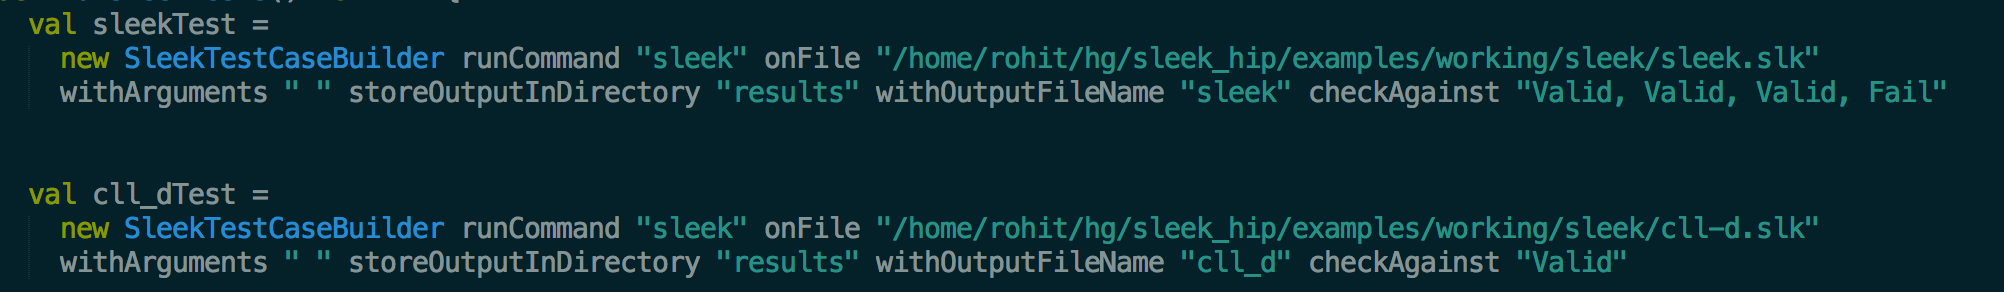
\includegraphics[width=500px]{figures/DSL_create_test.png}
  \caption{Individual Test Case Creation}
\end{figure}

\begin{figure}[h!]
  \centering
    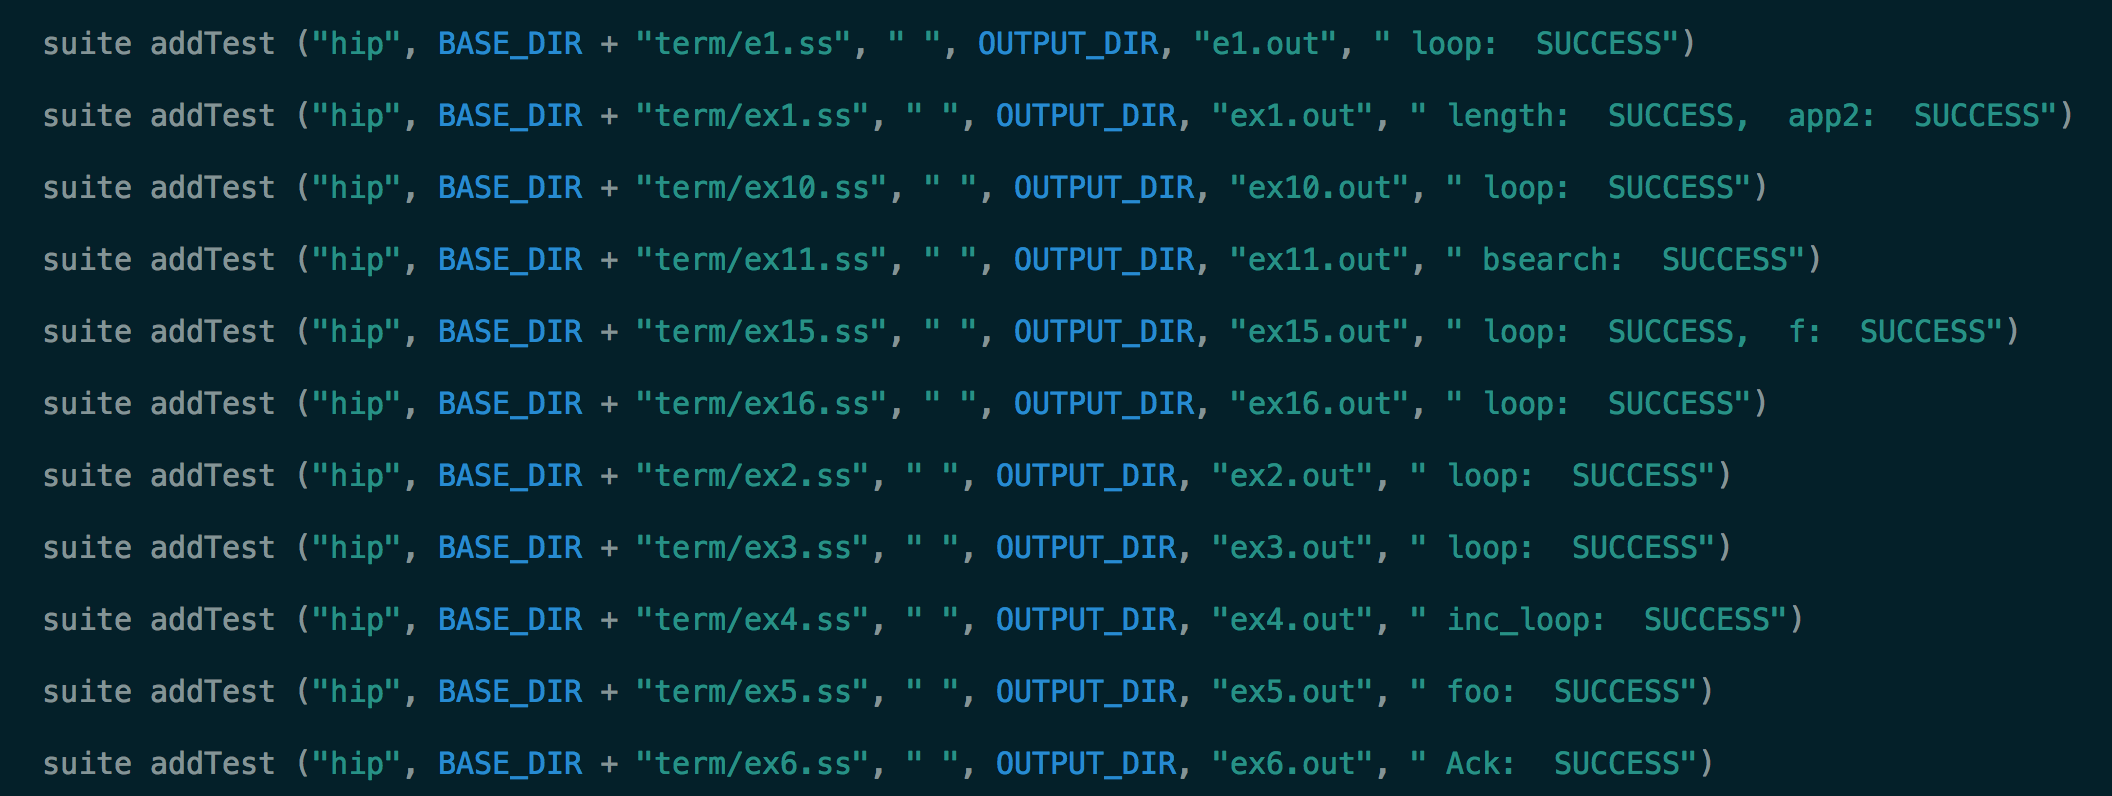
\includegraphics[width=500px]{figures/DSL_test_suite.png}
  \caption{Individual Test Suite Creation}
\end{figure}

\newpage
\subsection{Reporting/Scheduling Tool in Python}
A Reporting tool in Python was built over the course of the project. The Reporting tool performs the following functions:
\begin{itemize}
\item Test different commits in a project
\item Test different branches in a project
\item Prepare test reports
\end{itemize}

\subsection{Advantages of my solution}
\begin{itemize}
\item \textbf{Extensibility} - The embedded DSL is well documented using ScalaDoc and types are well defined and loosely coupled. Several design patterns such as \textit{Dependency Injection, Builder, Factory and Singleton} have been applied to make the code easier to extend and maintain
\item \textbf{Highly Configurable} - Both the embedded DSL and the Reporting Tool can be easily configured using \textit{human - readable} files. Scala's \textbf{config} type has been used to configure it whereas the reporting tool in Python can be configured using a YAML file.
\item \textbf{Lightweight Library} - The DSL has been implemented as a library that can be easily dropped into any project by including the .JAR in the project path. Dependencies are managed using sbt (Simple Build Tool).
\item \textbf{Easy to use} - The tools are very easy to configure and use because of the library approach and decoupled design.
\item \textbf{Domain Agnostic} - Although the DSL is currently used for hip/sleek verification and regression testing, it can be applied to any application for testing
\item \textbf{Integration with Version Controlled Workflow} - The output generated by the system is hierarchical and can be version controlled to create a repository of results.
\end{itemize}

% \newpage
% \subsection{Key Takeaways}
% \newpage

\newpage
\section{Literature Review}
There are several ways of designing and implementing Domain Specific Languages, each way having several merits and demerits. One of the most fundamental ways of classifying DSLs are Internal and External. \textbf{Internal DSLs} use the infrastructure of existing programming languages and build domain - specific constructs on top it. \textbf{External DSLs} are developed ground up and has separate infrastructure for lexical analysis, parsing, interpretation and compilation. In this project, we are restricting ourselves to internal or embedded DSLs on the host language of Scala.
\bigskip

\subsection{Research Methodology}

The research methodology followed during the project involved reading relevant papers, reading industry best practices and white - papers and iteratively building a suitable solution. Each iteration was approximately two weeks long and involved getting feedback from the users.

\begin{figure}[H]
  \centering
    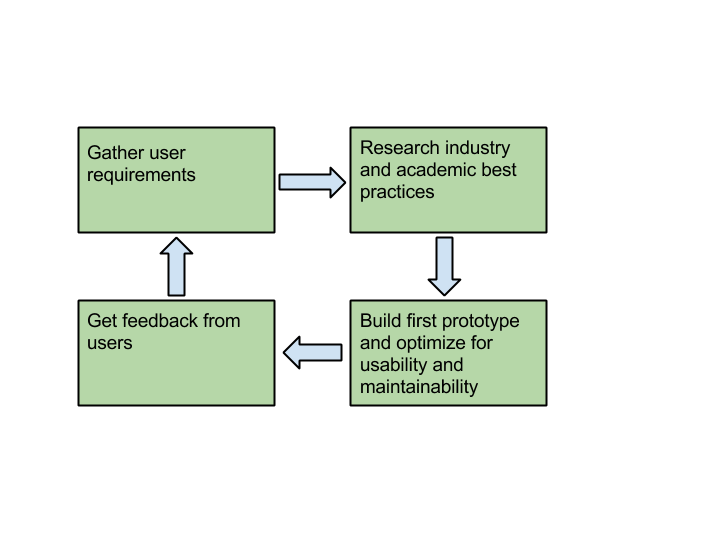
\includegraphics[height=300px]{figures/research.png}
  \caption{Research Methodology}
\end{figure}

\subsection{Testing Paradigms}
Release cycles and deployment cycles are becoming more and more frequent in the software engineering world and development teams are looking for reliable ways of testing their code's safety and functionality reliably and conveniently. Instituting an automated unit testing practice across a large software development team can be technically challenging and time consuming. Microsoft conducted a research study where a team of developers were instructed to write \textbf{unit tests} for all the functionality they wrote every 2 - 3 days. The bugs per unit of code were much fewer but there was a need for system level tests and integration tests \cite{unitTestingAtMicrosoft}. The chart below depicts the developer perception of the effectiveness of unit tests. The majority of Microsoft developers  are neutral towards unit testing.
\bigskip

\begin{figure}[H]
  \centering
    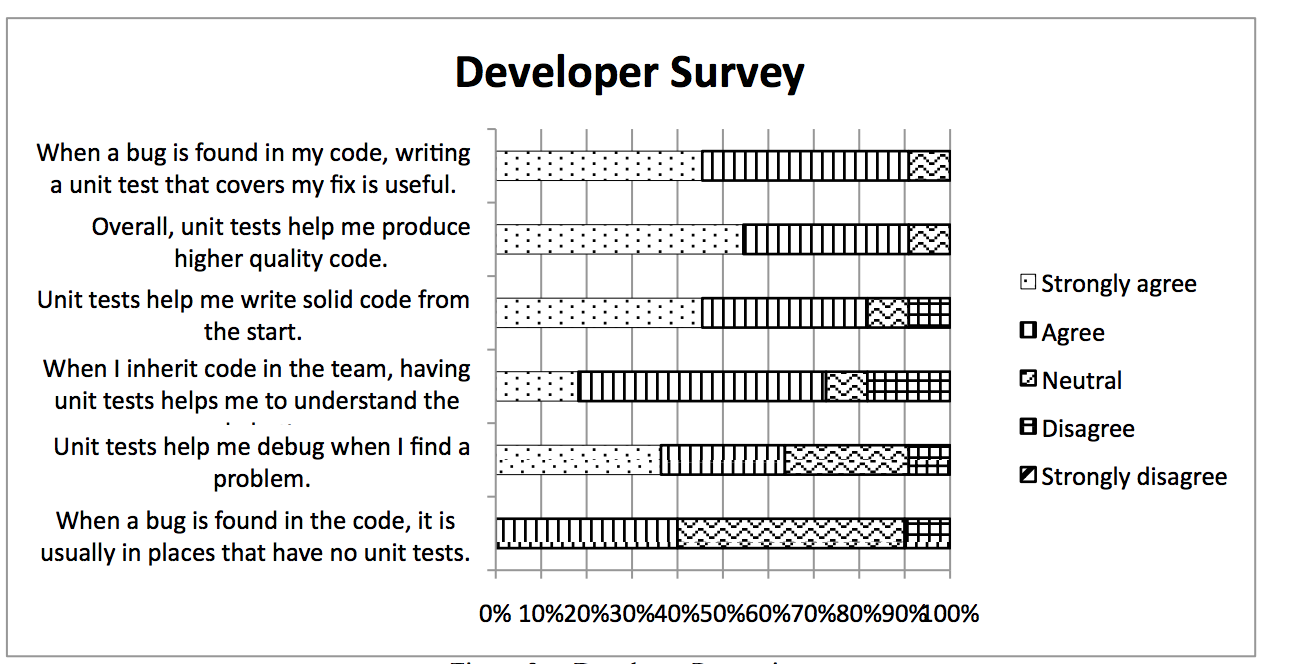
\includegraphics[height=200px]{figures/developer_perception.png}
  \caption{Developer Perception of the Effectiveness of Unit Testing}
\end{figure}

\noindent
In order to go beyond unit tests and perform functional tests at a system level, the DSL developed allows functional tests to be written for all kinds of domains. Since sometimes only the functionality of the software module is of primary concern, functional testing is used. Functional Testing is a testing method emphasized on executing the functions and examination of their input and output data \cite{Hetzel88}. Given the high proliferation of frameworks like \textbf{JUnit, ScalaTest and NUnit} for unit testing, a DSL for functional testing on the system testing was developed during this project. Hetzel also emphasizes the importance of regression testing since software is built as a composition of third - party libraries and in - house components. This dictates that any minor change should lead to re - running tests on a unit level \cite{Hetzel88}. Therefore, the DSL developed has extensive support for \textbf{regression testing and reporting}.

\subsection{Domain Specific Language Design}
Ghosh discusses two approaches to constructing internal DSLs - \textbf{Embedded} and \textbf{Generative} \cite{dslsInAction}. Statically typed languages offer types as one of the means to abstract domain semantics and make the surface syntax of the DSL concise. Typed models come with a
guarantee of some level of implicit consistency in the programming model. The biggest advantage of this technique is that because the DSL’s type system is embedded in the type system of the host language, the type system is automatically type-checked by the language compiler. This approach means that DSL users are able to use the IDE for debugging and tooling. In our System Testing DSL, this embedded DSL approach has been explored. 
\bigskip

\begin{figure}[H]
  \centering
    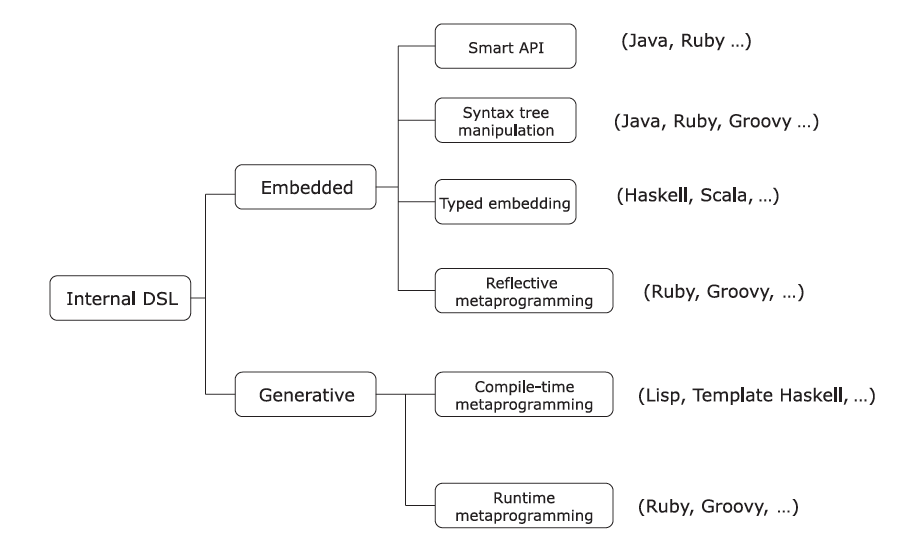
\includegraphics[height=250px]{figures/classification.png}
  \caption{Micro - classification of DSLs}
\end{figure}

\noindent
Languages like Haskell and Scala offer advanced static typing with type inference allowing DSL developers to write embedded DSLs without having to resort to code generation techniques, pre - processors or macros. As a DSL user, type abstractions can be composed directly. This is the approach that has been taking while writing the System Testing DSL. Ghosh talks about using method chaining and fluent interfaces in DSL development as this gives a finished, declarative, natural language like feel \cite{fluentInterface}. The builder pattern is one more way in which DSL's can be made more expressive to the domain user. The builder pattern along with method chaining have been incorporated into the System Testing DSL to provide ease of use and expressiveness.

\subsection{Lightweight Modular Staging: A run - time code generation approach}
Rompf and Odersky (2010) talk about an alternative approach to writing DSLs in Scala using a run - time code generation approach called lightweight modular staging \cite{lms}. This approach involves both a generative and an embedded approach. The DSL is provided as a library and involves run - time code generation in different stages. The approach is called \textbf{Light - Weight Modular Staging (LMS)}. The approach is lightweight because the whole framework is implemented as a library and the staged code is very shallowly embedded into the program generator. Some of the features of lightweight modular staging are described below:
\begin{itemize}
\item Immediate/deferred compilation of certain objects are distinguished by type
\item The Scala language is expressive enough to allow the framework to be implemented as a library
\item staged code is “very shallowly” embedded into the program generator
\end{itemize}
\bigskip

\noindent
Lightweight modular staging provides many of the benefits of using a dedicated multi-stage programming language such as MetaOCaml, in particular concerning well-formedness and type safety, but goes beyond that in systematically preventing code duplication and providing a clean interface for incorporating generic and customized optimizations. However, after careful evaluation, this method was not chosen as the project is still not mature enough and different focus of the project.

\subsection{Delite: A framework for high - performance DSL's}
A third approach to writing embedded, high - performance DSLs conducted by Odersky built upon the concept of using lightweight modular staging. The research resulted in a framework called Delite \cite{delite}. Delite's compilation pipeline takes care of optimizing for target hardware such as multi - core processors, GPUs and computing clusters.

\begin{figure}[H]
  \centering
    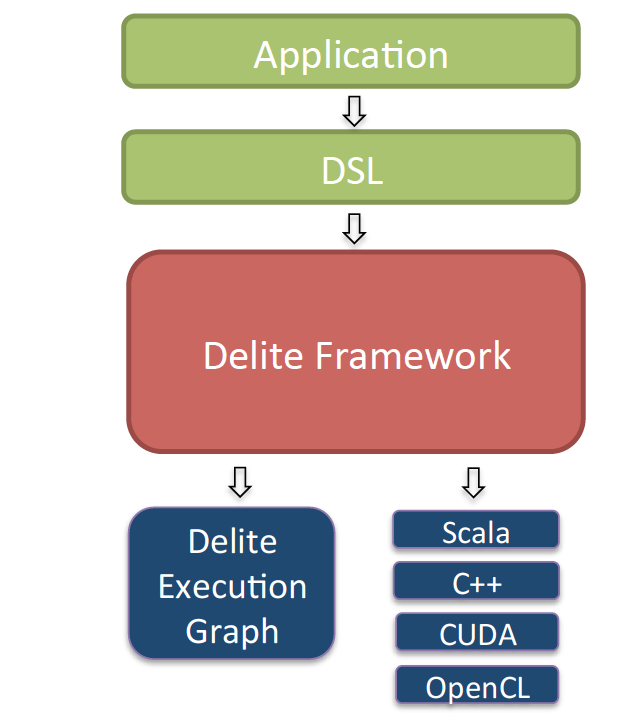
\includegraphics[width=170px]{figures/delite.png}
  \caption{Delite Framework Overview}
\end{figure}

\noindent
In the early stages of this project, the Delite framework was experimented with to gauge the suitability of the framework in everyday DSL development. However, due to the lack of sufficient tooling and documentation - the plans of using Delite were set aside till the next semester of research so that better support and documentation is available.
\bigskip

\subsection{Scala programming language}
The \textbf{Scala} programming language was chosen as the host language for the DSL being developed. Scala is extremely well - suited for building embedded DSLs with custom syntax and rich type systems. Compiler features such as an \textbf{extensible type system, flexible syntax, type inference and static typing} are just some of the primary reasons for using Scala. According to the Scala specification, \textit{Scala is a statically typed multi-paradigm language that attempts to unify object-oriented and functional programming} \cite{scala}
\bigskip

\noindent
A recent paper published by Google comparing the performance of Scala, Java and Go show that although Scala has greater compilation times than Java and Go, the lines of code in Scala to achieve similar tasks are much lower than Java or Go. This is one more reason why Scala is suitable for DSL programming \cite{performanceComparison}.

\begin{figure}[H]
  \centering
    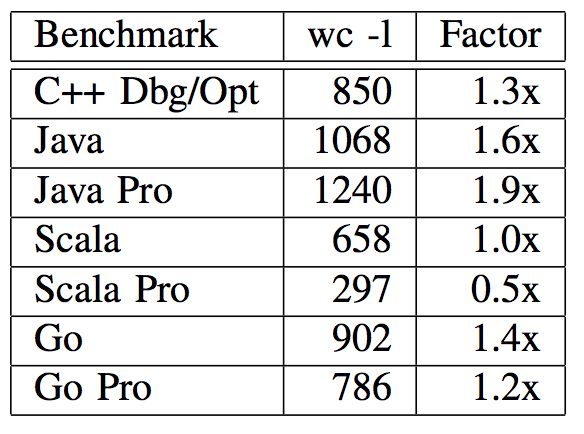
\includegraphics[height=150px]{figures/scala_loc.png}
  \caption{Comparison of Scala lines of code with other languages}
\end{figure}

\subsection{Python programming language}
Along with the DSL in Scala, a reporting tool was built for running tests on different branches of a \textbf{mercurial} project and then summarizing the results in a convenient directory structure. This reporting tool was built in Python and is configured using YAML markup. The reason for choosing python was:
\begin{itemize}
\item It is a dynamic language and well - suited for such systems
\item It is close to the operating system and can easily make system calls
\item It supports \textbf{object orientation} leading to a more modular design \cite{python}
\end{itemize}

\begin{figure}[H]
  \centering
    
\includegraphics[height=150px]{figures/python_lang.png}
  \caption{Python}
\end{figure}
After consideration of these factors, \textbf{Python} was chosen to build the system with a configuration file written in YAML.

\subsection{Approach Chosen}
Out of the three DSL design approaches explored - \textbf{DSL development using embedded types}, \textbf{Lightweight Modular Staging} and \textbf{The Delite Framework}, the first one was chosen for developing the System Testing DSL. The choice was made so that we could gain an understanding of the types and usage required in the DSL and could build a suitable DSL for the problem domain identified - \textit{System Testing}.
\bigskip

\noindent
\textbf{Scala} was chosen as the DSL host language and \textbf{Python} as the host language for the reporting and scheduling tool. The two tools can interact closely using a \textbf{configuration file written in YAML}. However, they are decoupled and can be just as easily be used in isolation.
\newpage

\section{DSL/System Details}

\subsection{Source Code}
The code for this project and related documentation can be found in the repository below on the master branch.\newline
\textbf{Link:} https://github.com/rohitmukherjee/High-Performance-DSLs

\subsection{Overview of System}
Over the course of this year, a DSL for system testing was developed using Scala as the host language. It can be used for testing any set of executables/applications and match their generated console output against specified values or rules. The language can also be used to check whether the system is operational or not.
\bigskip

\noindent
\textbf{Regression Testing} is also one of the key features of the DSL. Users can generate \textbf{reference tests} with a certain ideal set of data and then run tests against the \textbf{regression reference} conveniently. All the test specific details can be configured using a configuration file - \textbf{application.conf}. This allows users to write regression tests without writing any code and just specifying certain settings in plain text.
\bigskip
\begin{figure}[H]
  \centering
    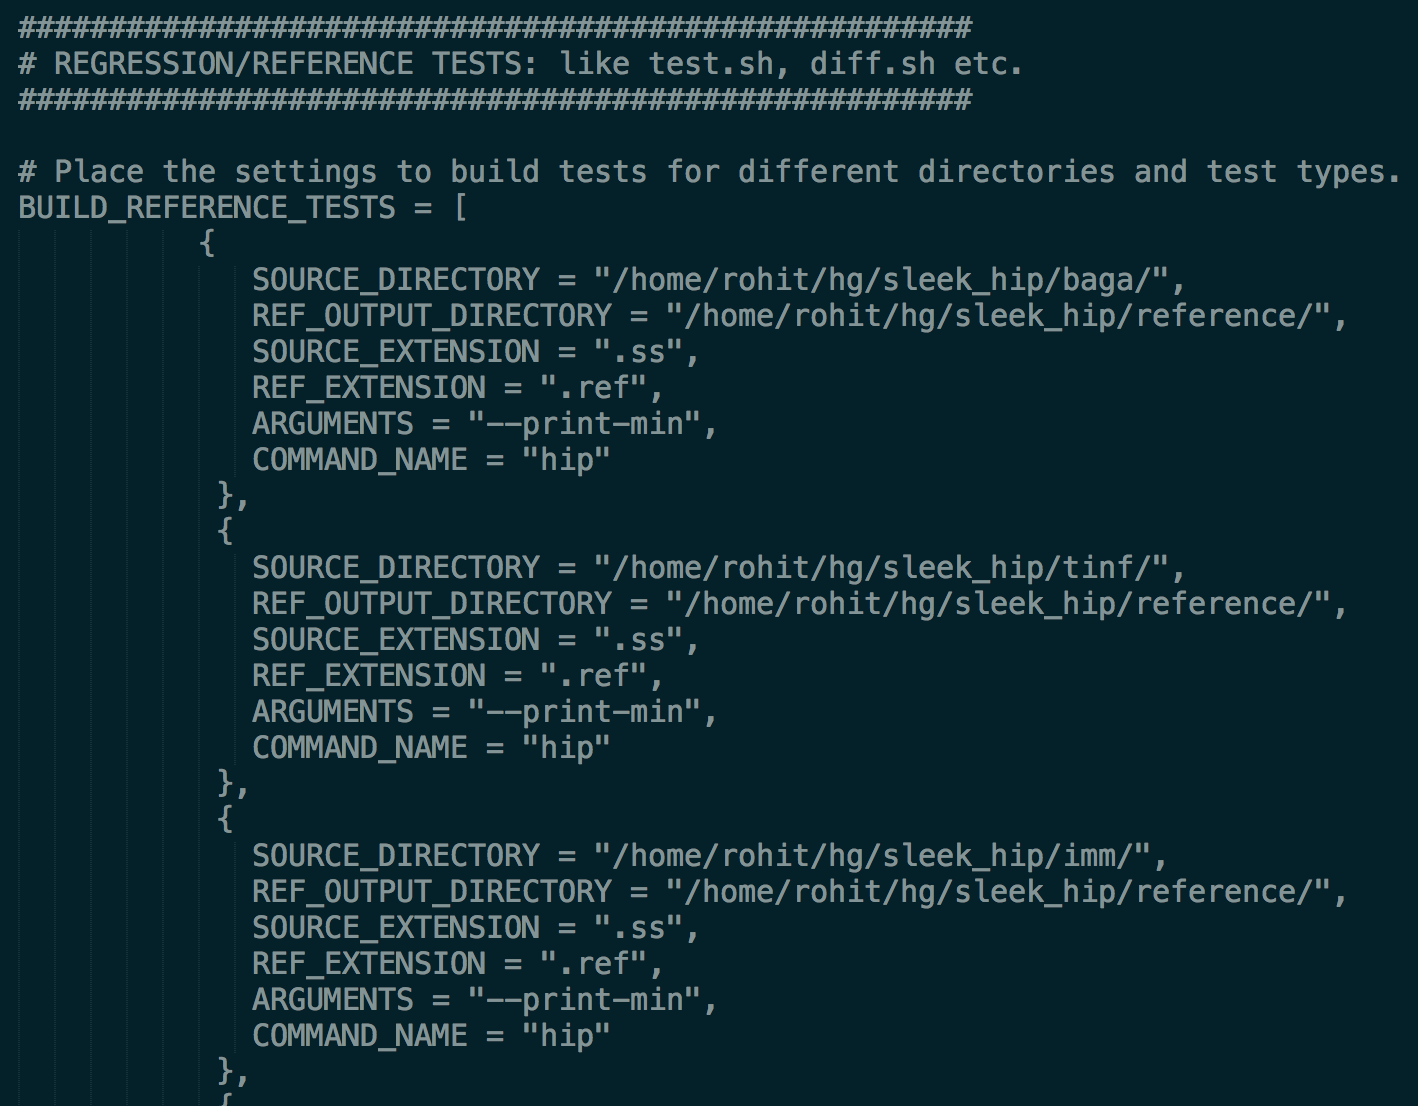
\includegraphics[height=250px]{figures/application_conf.png}
  \caption{application.conf - the driver for regression tests}
\end{figure}

\noindent
For regression testing there are 3 primary options provided  - \textbf{buildReference, runReference and overrideReference}. The first one creates a repository of reference results for specified tests. The second option runs a set of tests against the stored references. The last option is for selectively rebuilding reference results. For example, a certain test in a test suite may have changed so it's reference result has to be changed.
\bigskip

\begin{figure}[H]
  \centering
    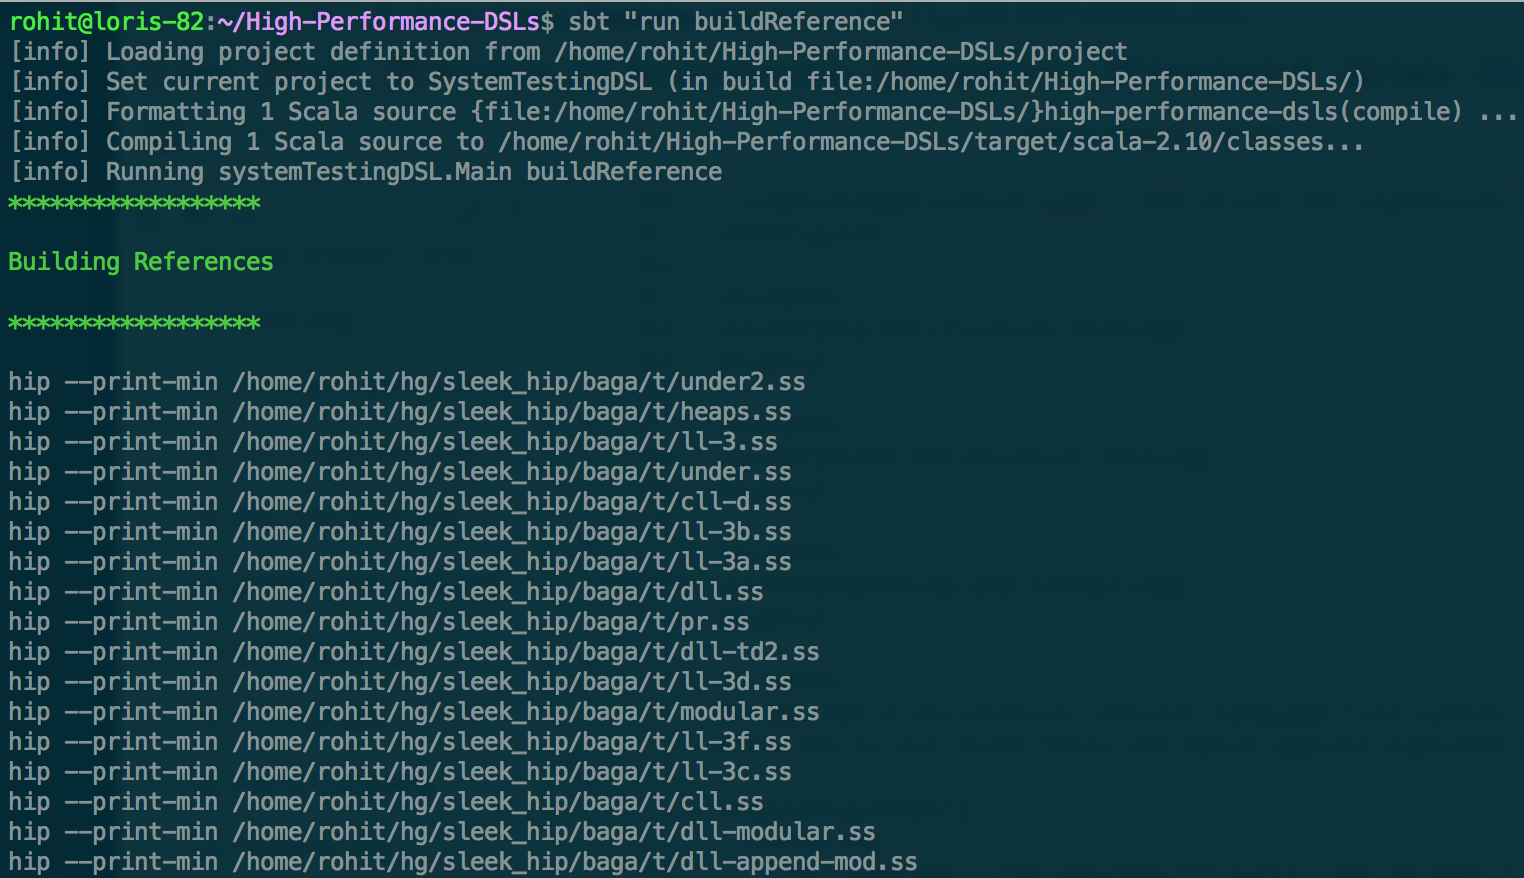
\includegraphics[height=300px]{figures/building_reference.png}
  \caption{Building References for Regression Testing}
\end{figure}

\noindent
\textbf{Hip Verification Testing} was one of the first applications of the DSL. The \textbf{HIP/SLEEK} systems are aimed at automatic verification of functional correctness of heap manipulating programs. HIP is a separation logic based automated verification system for a simple imperative language, able to modularly verify the specifications of heap-manipulating programs \cite{hipsleek}. The DSL developed can perform HIP lemma testing. Running with the option \textbf{"hip"} tests the hip files. The screen - shot below shows the hip tests running. Coloured console output showing outcome is shown.
\bigskip

\begin{figure}[H]
  \centering
    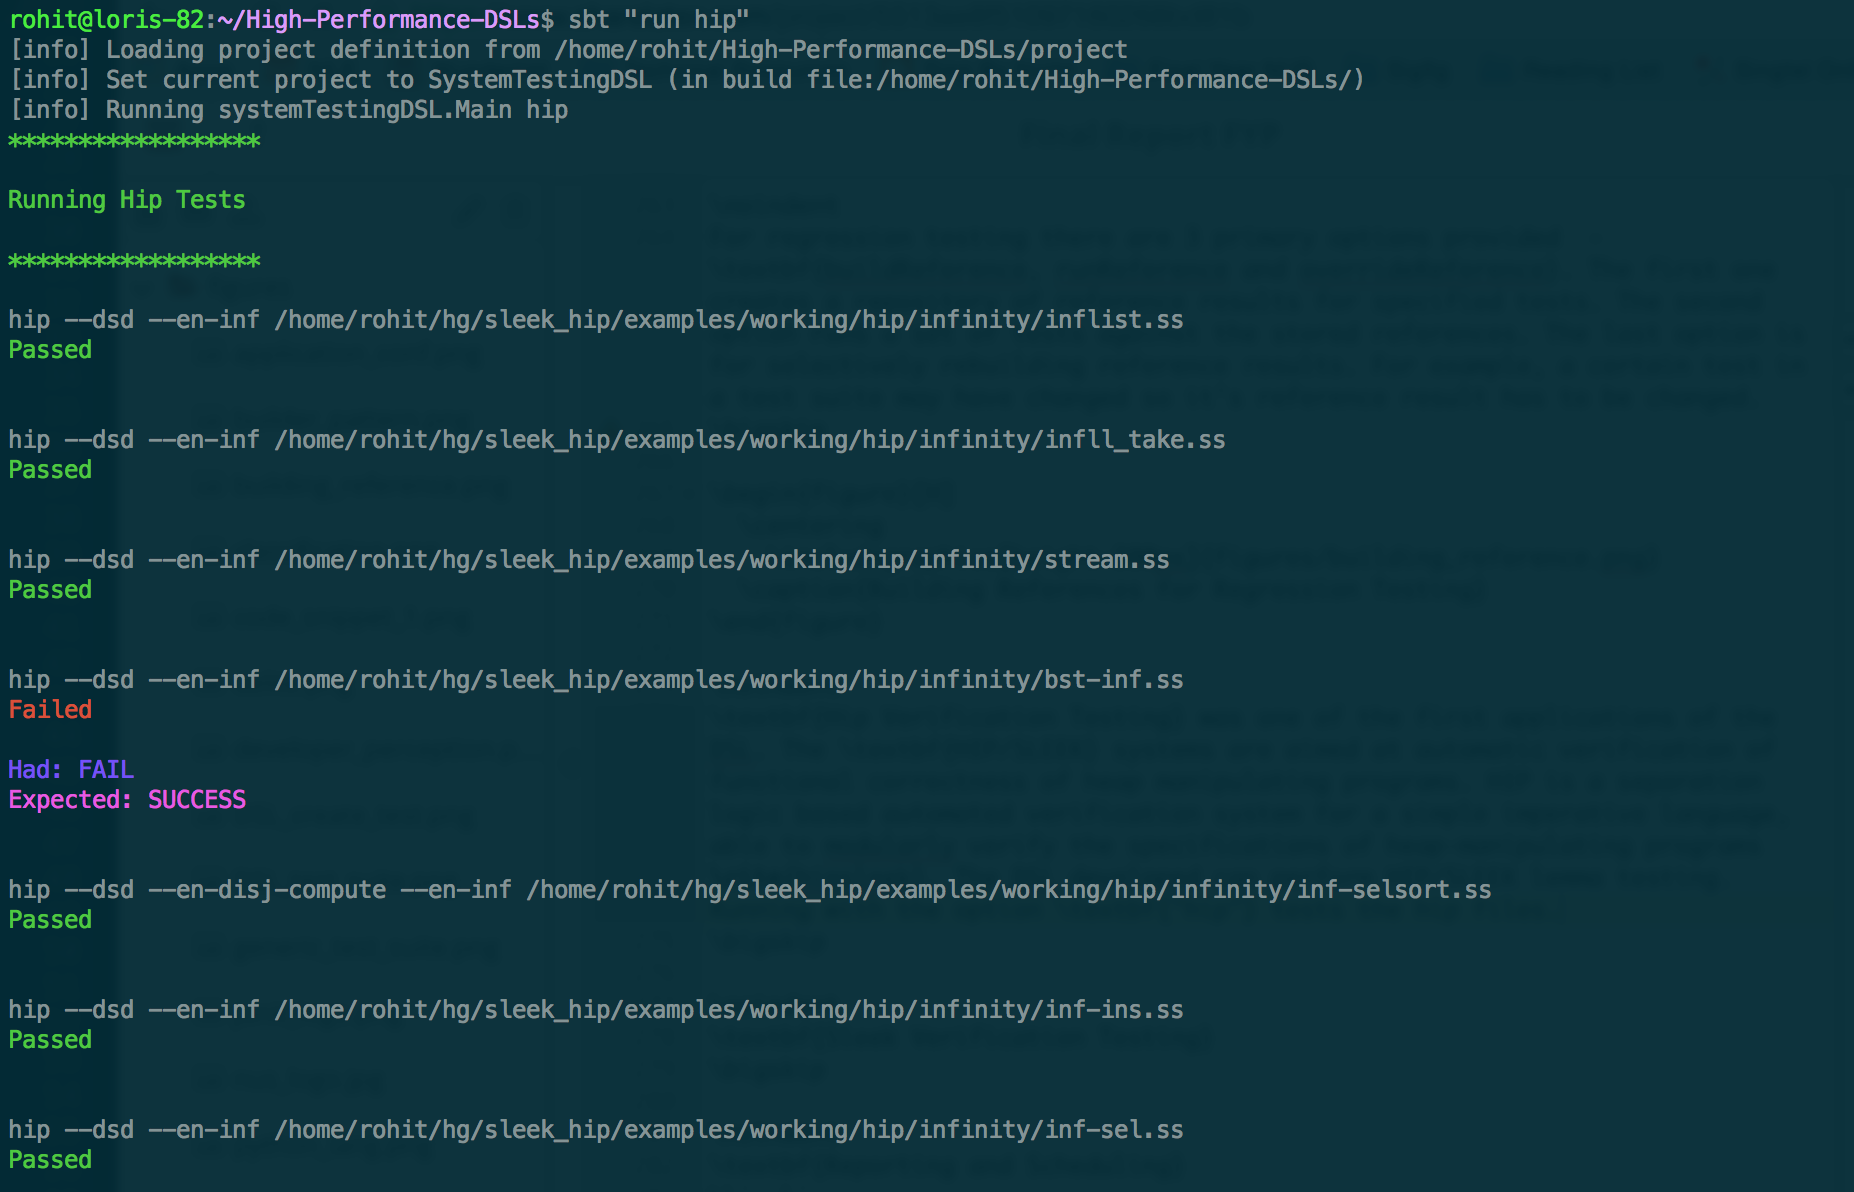
\includegraphics[height=300px]{figures/hip_testing.png}
  \caption{Running Hip Tests}
\end{figure}

\noindent
\textbf{Sleek Verification Testing} is also one of the main applications of the DSL currently. The various Sleek Entails can be verified by running the \textbf{sleek} option in the DSL. The DSL uses specific \textbf{regular expressions} and \textbf{parsing rules} to ascertain whether an entail has been correctly passed or failed. The DSL provides extensibility in terms of output produced. It has \textbf{Console output} and \textbf{HTML output} capabilities allowing the system to produce \textbf{browser - friendly content}.
\bigskip

\begin{figure}[H]
  \centering
    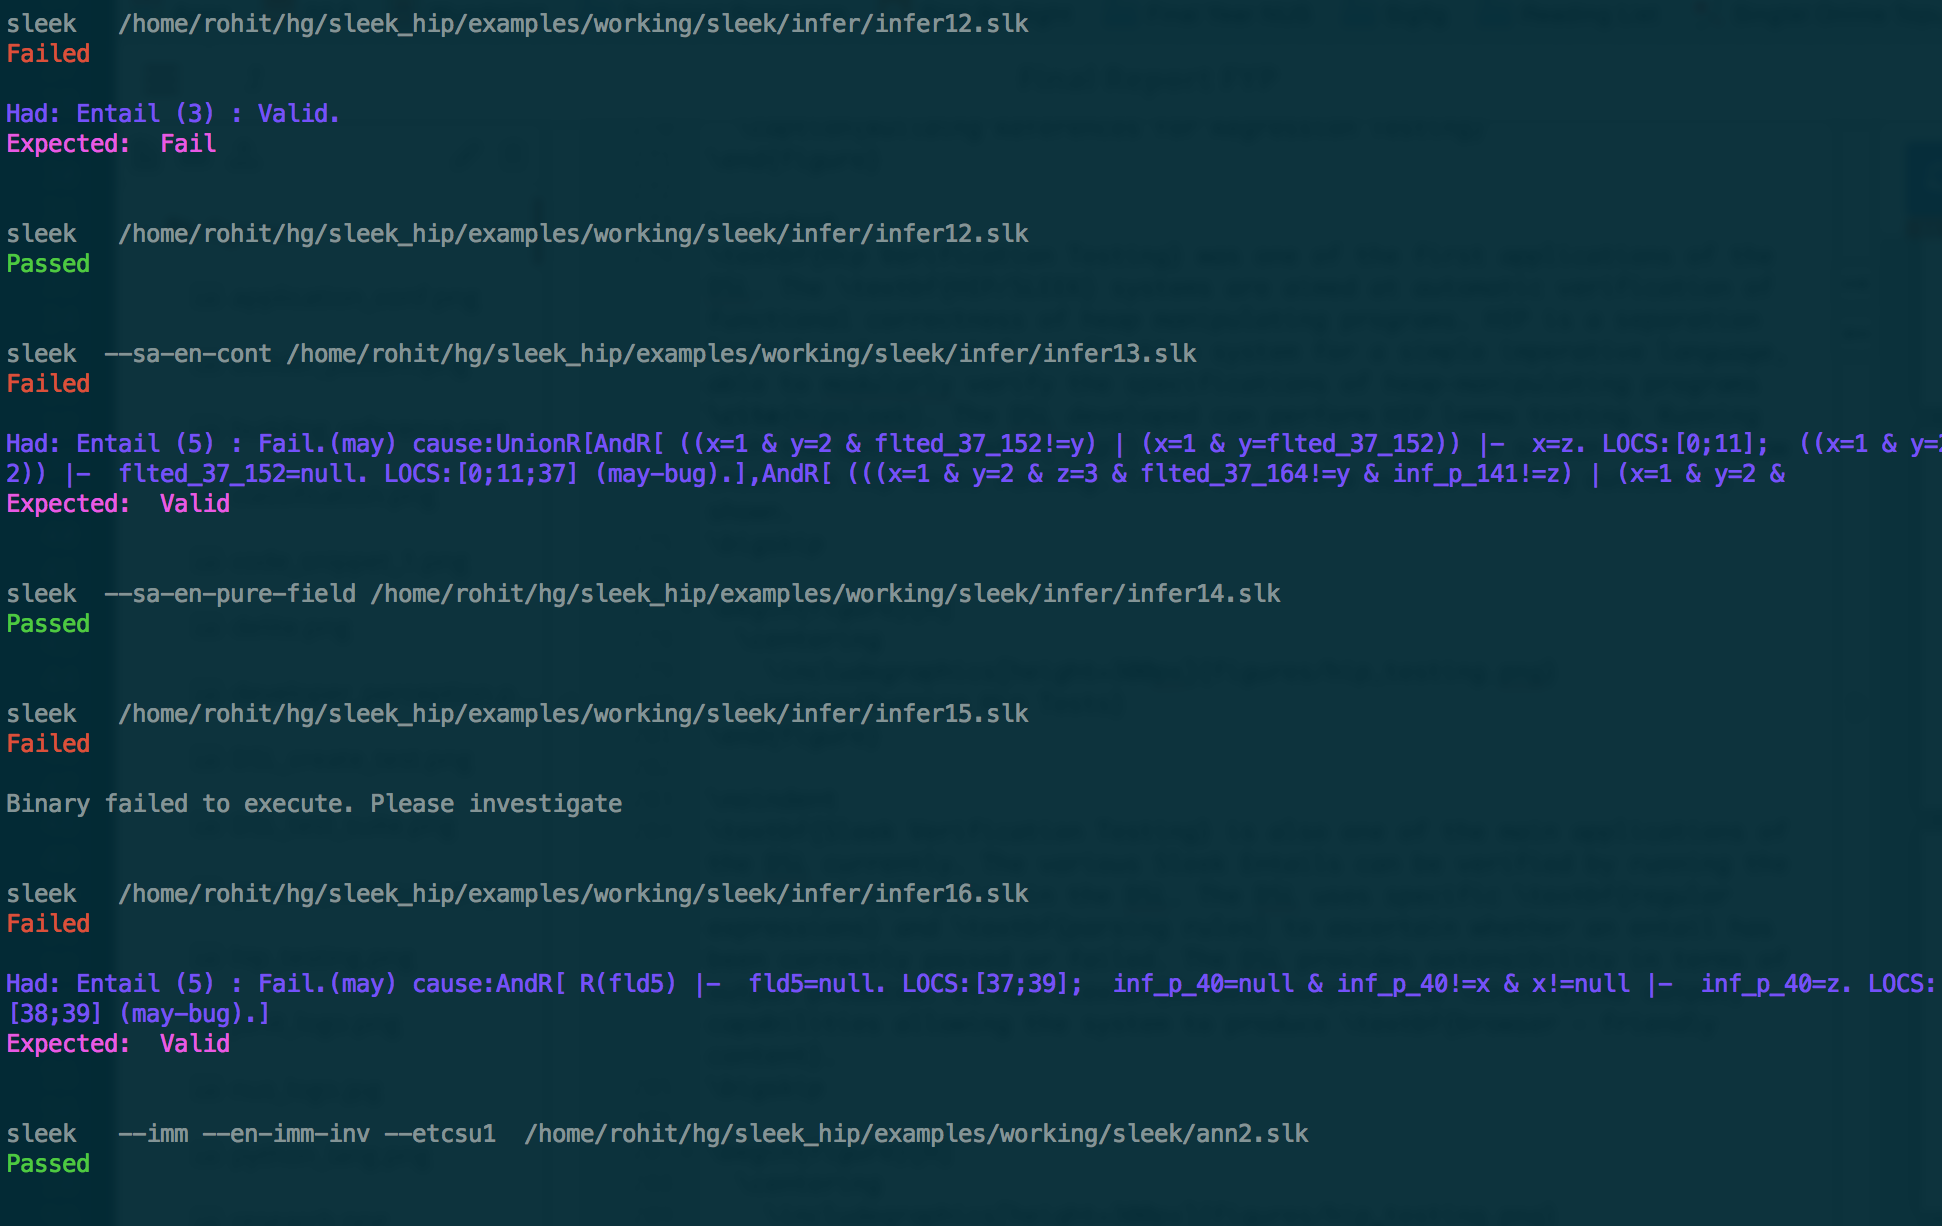
\includegraphics[height=300px]{figures/sleek_testing.png}
  \caption{Running Sleek Tests}
\end{figure}

\noindent
After running all the tests, \textbf{test statistics} are produced in addition to \textbf{logged output}. \textbf{JUnit} was the inspiration for such a command line interface.

\begin{figure}[H]
  \centering
    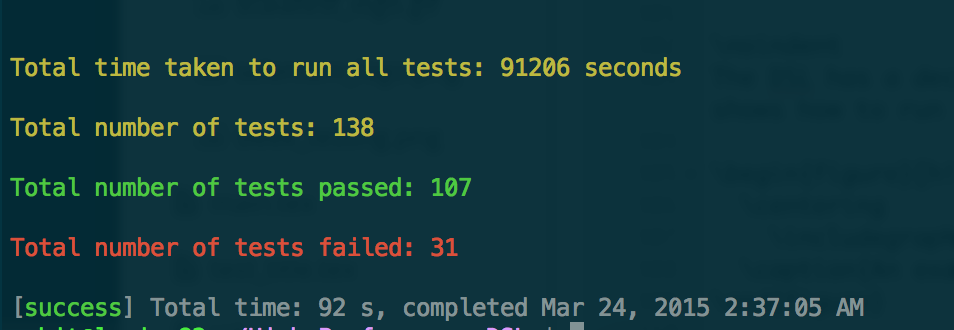
\includegraphics[height=150px]{figures/test_statistics.png}
  \caption{Test statistics at the end of every test}
\end{figure}

\noindent
\textbf{Reporting and Scheduling} are two features that are decoupled from the core DSL and are written in \textbf{Python}. The Python tool is responsible for doing the following:
\begin{itemize}
\item Check out individual branches of a mercurial repository
\item Run the DSL's tests (sleek/hip/regression) against each branch
\item Summarize the results conveniently in a hierarchical directory
structure
\item Run tests against each commit as long as it is a new commit (users can define what they mean by "new" using a \textbf{settings.yaml } file)
\end{itemize}

More details on how this tool is built and works can be found in the \textbf{Overview of Python Code} section.
\bigskip


\newpage
\subsection{Software Engineering Methodology}

The project was built over the period of one year following certain software engineering methodologies. Some of these methodologies are:
\begin{itemize}
\item \textbf{Test Driven Development (TDD)}: Test-driven development (TDD) is a software development process that relies on the repetition of a very short development cycle: first the developer writes an (initially failing) automated test case that defines a desired improvement or new function, then produces the minimum amount of code to pass that test \cite{tdd}. Tests for the DSL can be found in \textbf{src/test/scala/systemTestingDSL/} and can be executed by running \textbf{"sbt test"}.

\begin{figure}[H]
  \centering
    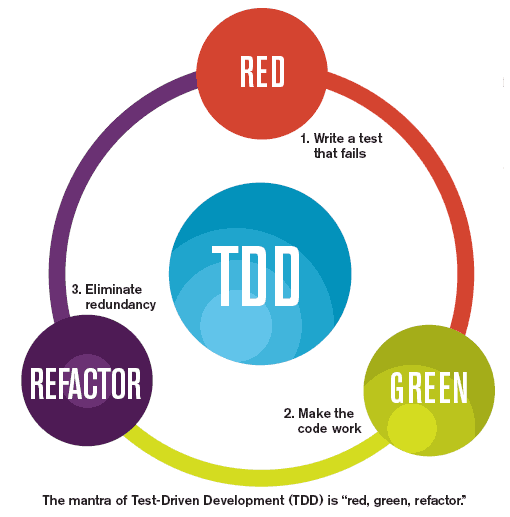
\includegraphics[height=130px]{figures/tdd.png}
%   \caption{}
\end{figure}

\item \textbf{Agile Software Development}: Agile development provides opportunities to assess the direction throughout the development life - cycle. Every few days (in this case 2 weeks), new features are shown to the users and based on feedback and criticism from them, changes are made. This process is continued throughout the entire life - cycle of the project ]\cite{agile}.

\begin{figure}[H]
  \centering
    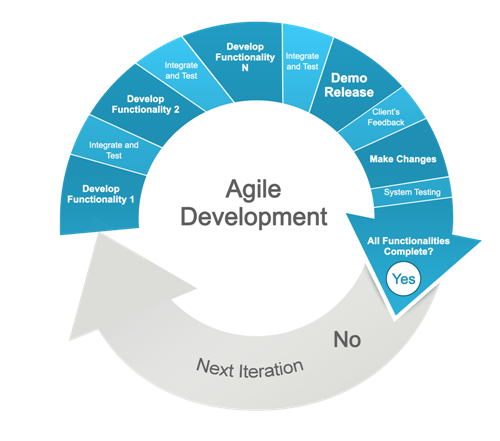
\includegraphics[height=150px]{figures/agile.png}
  \caption{Agile explained}
\end{figure}
\end{itemize}

\newpage
\section{Design Choices}

Some of the primary design choices in the project are summarized below:

\subsection{Architecture of System}

\subsection{Choice of Scala as Host Language}
\textbf{Choice of Scala as host language}: The adoption of Scala has grown tremendously over the last 5 years in the industry with large organizations such as Twitter, Bank of America Merrill Lynch and Groupon using it for DSL design \cite{scala}. The expressive syntax and intelligent type inference allows a clean domain syntax and type system to be developed. Portability of code because of the JVM platform is another factor promoting Scala's adoption \cite{scala}. The reasons for using Scala are summarized below:

\begin{figure}[H]
  \centering
    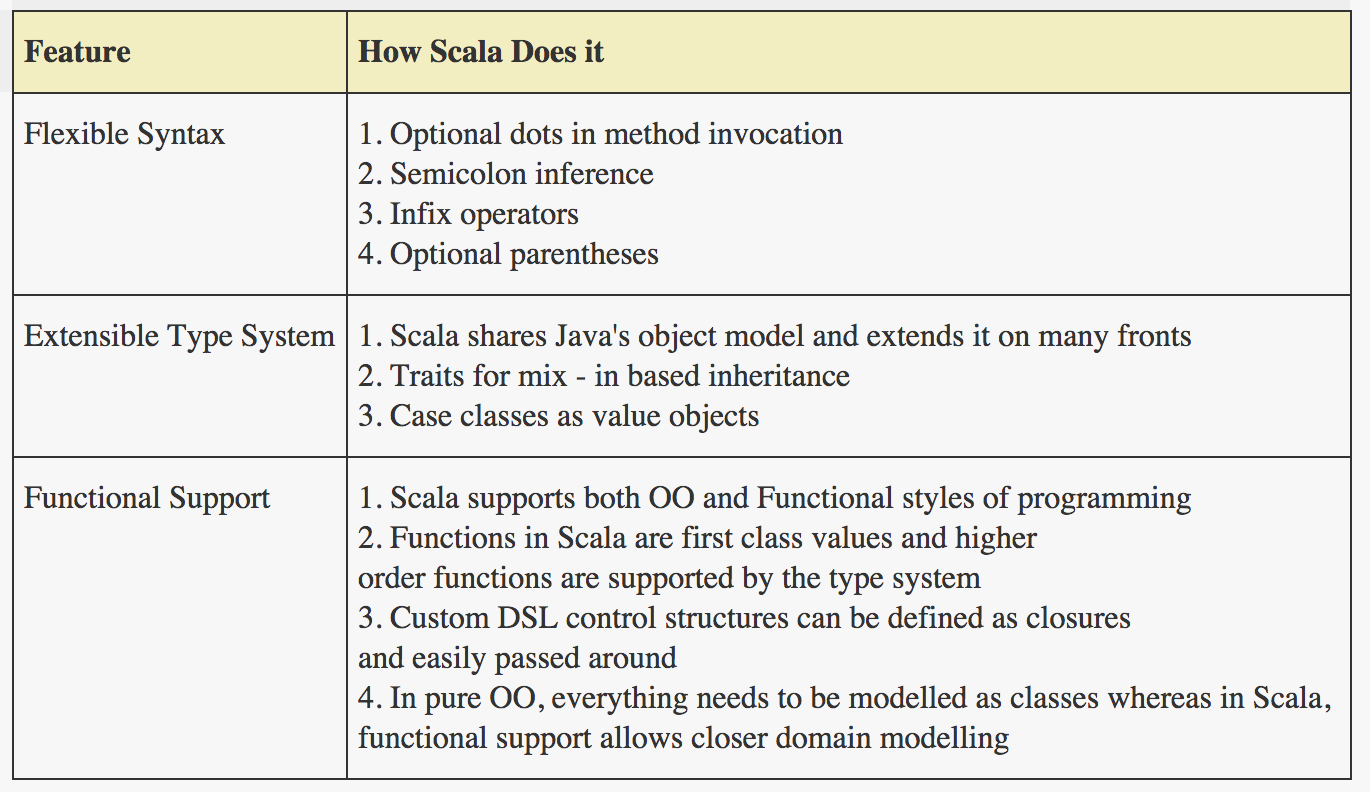
\includegraphics[width=500px]{figures/scala_motivation.png}
  \caption{Motivation for using Scala}
\end{figure}

\subsection{Choice of Python for Reporting Tool}

After careful evaluation of possible options for developing the reporting tool, \textbf{Python} was chosen as the implementation language. The functionality desired in the reporting tool was as follows:
\begin{itemize}
\item Check out different commits for a particular \textbf{mercurial} branch
\item Check out different branches for a particular \textit{mercurial} repository
\item Ease of configuring system and ability to hot - switch settings during run - time
\item \textbf{Object Orientation} for readability and maintainability
\item Ability to run tests on all branches/commits and report results reliably
\end{itemize}

\noindent
\textbf{Dynamic languages}, such as Python, Ruby, Dylan, LISP, Scheme, and Smalltalk, are languages designed to increase programmer efficiency. Dynamic
languages enables faster development cycles by allowing parts of a program to be modified at run time. Functions may be introduced, removed, or changed, classes added, class inheritance modified, and modules can be created or removed. This allows a programmer to quickly test a new feature, or a new piece of code. Furthermore, modern dynamic languages, such as Python and Ruby, provide syntax and high-level programming models that are easy to learn, resulting in higher productivity \cite{lund}.
\bigskip

\noindent
Some of the reasons for using Python were:
\begin{itemize}
\item Object Orientation Support
\item Dynamic Language
\item Support for scripting
\item Lower development time
\item High readability
\end{itemize}

\subsection{Choice of Embedded DSL Approach}
Instead of starting off development using the Delite Framework or the Lightweight Modular Staging Library, I decided to write a DSL with an embedded type system and no run - time code generation or optimizations. This allowed me to understand the important types and constructs required in the domain and develop a clean syntax. It also allowed me to model the domain without concerning myself with lower level optimizations prematurely. Some of the advantages of creating an embedded DSL were:
\begin{itemize}
\item \textbf{Lightweight} - The DSL has been written as a \textit{library} which can be easily included in other projects by simply adding the .JAR file to the project build path.
\item \textbf{Compile time type checking} - Since there is no code generated at run - time or any meta - programming, all types are checked at compile - time giving us the added support of the Scala compiler.
\item \textbf{Easily maintainable and extensible} - Since the source code is written using the Scala language, it is readable and easily extensible if new functionality is desired. The system also follows the \textbf{open - closed} principle. It is open for extension but closed for modification.
\item \textbf{Emphasis on Semantics} - Domain rules can vary and can require extension or revision. It is very important that the DSL provides \textit{Pluggable semantics} according to Ghosh \cite{dslsInAction}. Appropriate usage of Scala types including \textit{traits, types and objects} make the semantics quite meaningful. For example, when we want to add a test, we can write syntax like:

\begin{figure}[H]
  \centering
    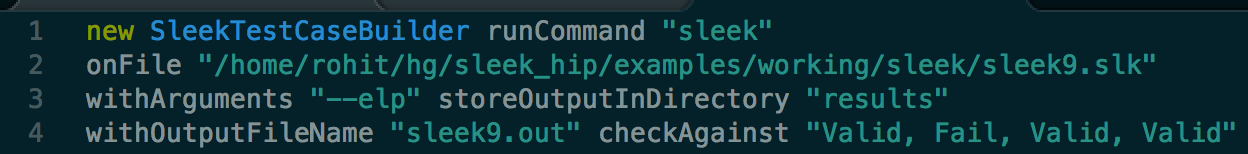
\includegraphics[height=60px]{figures/declarative_syntax.png}
  \caption{Meaningful Semantics}
\end{figure}

\item \textbf{Loose Coupling} - Loose coupling between the composed DSLs, and their rules, allowing all the rules to evolve independently.
\item \textbf{Representation Independence} - The DSL does not contain any embedded implementation details and merely shows domain abstractions.
\end{itemize}

\subsection{Design Pattern Choices}

Ghosh \cite{dslsInAction} talks about certain design patterns being industry "best - practices" for DSL development. Over the course of this project, these patterns have been used extensively:
\begin{itemize}
\item \textbf{Singleton Pattern} - For re - usable components like regex/file system utilities. Scala provides an \textbf{Object} type that implements this pattern without requiring any boilerplate code. An example of this pattern is shown below:

\begin{figure}[H]
  \centering
    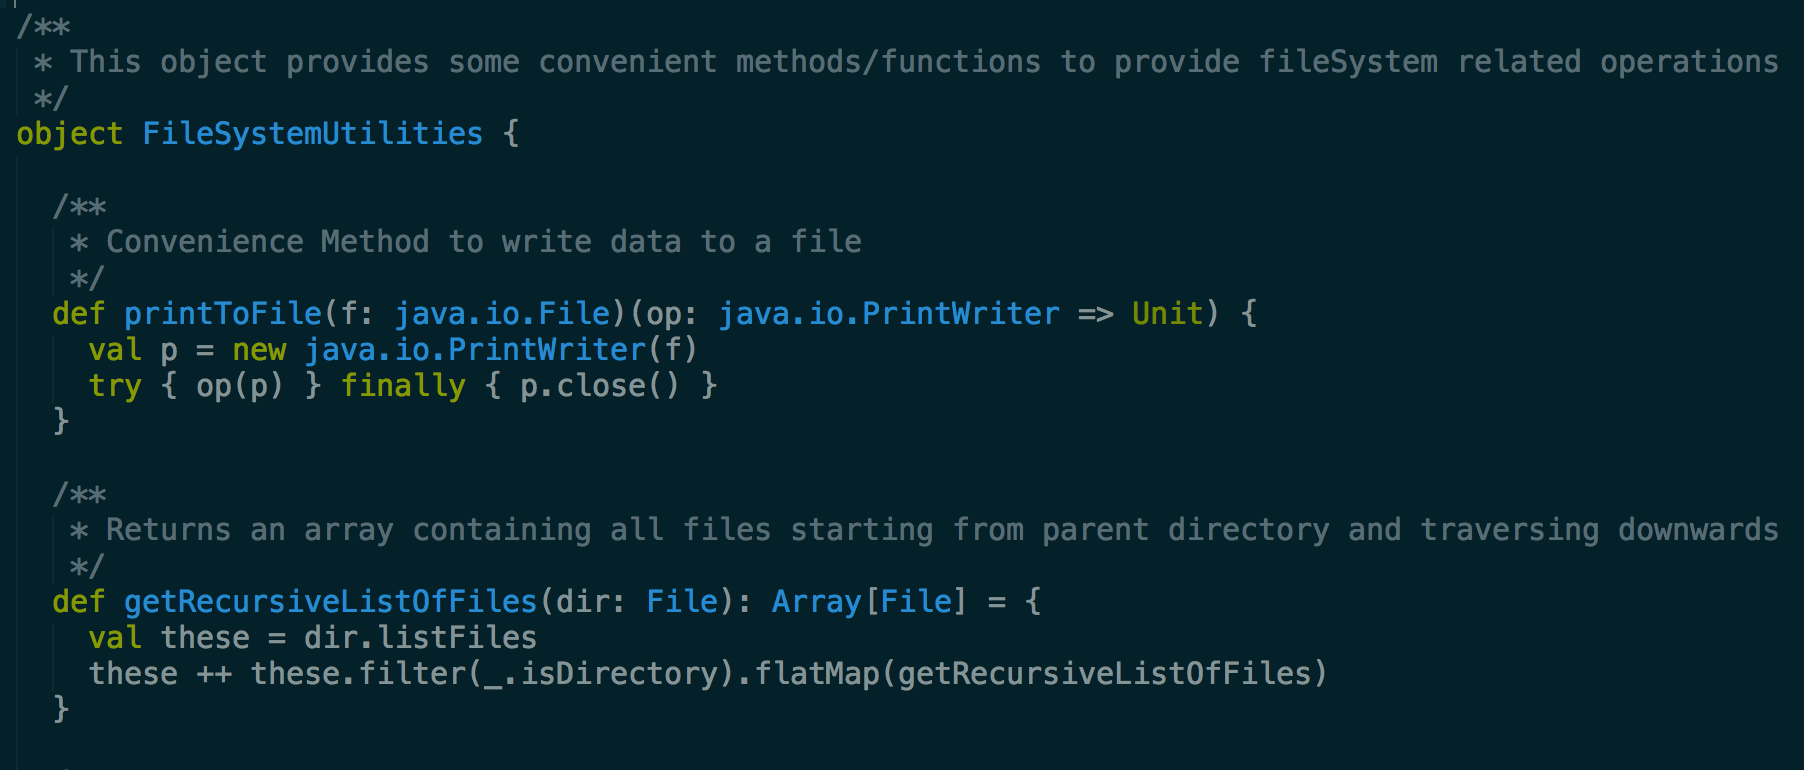
\includegraphics[width=500px]{figures/singleton.png}
  \caption{An example of Singleton pattern usage}
\end{figure}

\item \textbf{Builder Pattern} - Builder pattern builds a complex object using simple objects and using a step by step approach. This type of design pattern comes under creational patterns as this pattern provides one of the best ways to create an object. Our SLEEK/HIP tests are instantiated incrementally and therefore the builder pattern is natural choice. The builder pattern combined with the \textbf{fluent interface} concept gives the DSL a declarative feel.

\item \textbf{Factory Pattern} - This is used in the project by defining trait for creating an object, but let the classes that implement the interface decide which class to instantiate. The Factory method lets a class defer instantiation to subclasses. For context - aware choice of which kind of class to instantiate. This has been used to switch between \textbf{Console Output and HTML Output}.

\item \textbf{Future Timeout Design Pattern} - Scala Futures provide an elegant way of handling asynchronous operations in Scala \cite{scala}. They allow developers to write non - blocking processes running on a different thread. They allow us to wait on the thread for completion (which is actually an anti - pattern because we could have just used a blocking call), pass messages/arguments to the thread when it is done executing (\textit{Promises}) or just time - out after a certain duration (\textit{Awaits}). In this context, the time - out pattern using Awaits is being used to prevent processes from blocking indefinitely. This can be set by setting the \textbf{TIMEOUT} variable in the system configuration.
\begin{figure}[H]
  \centering
    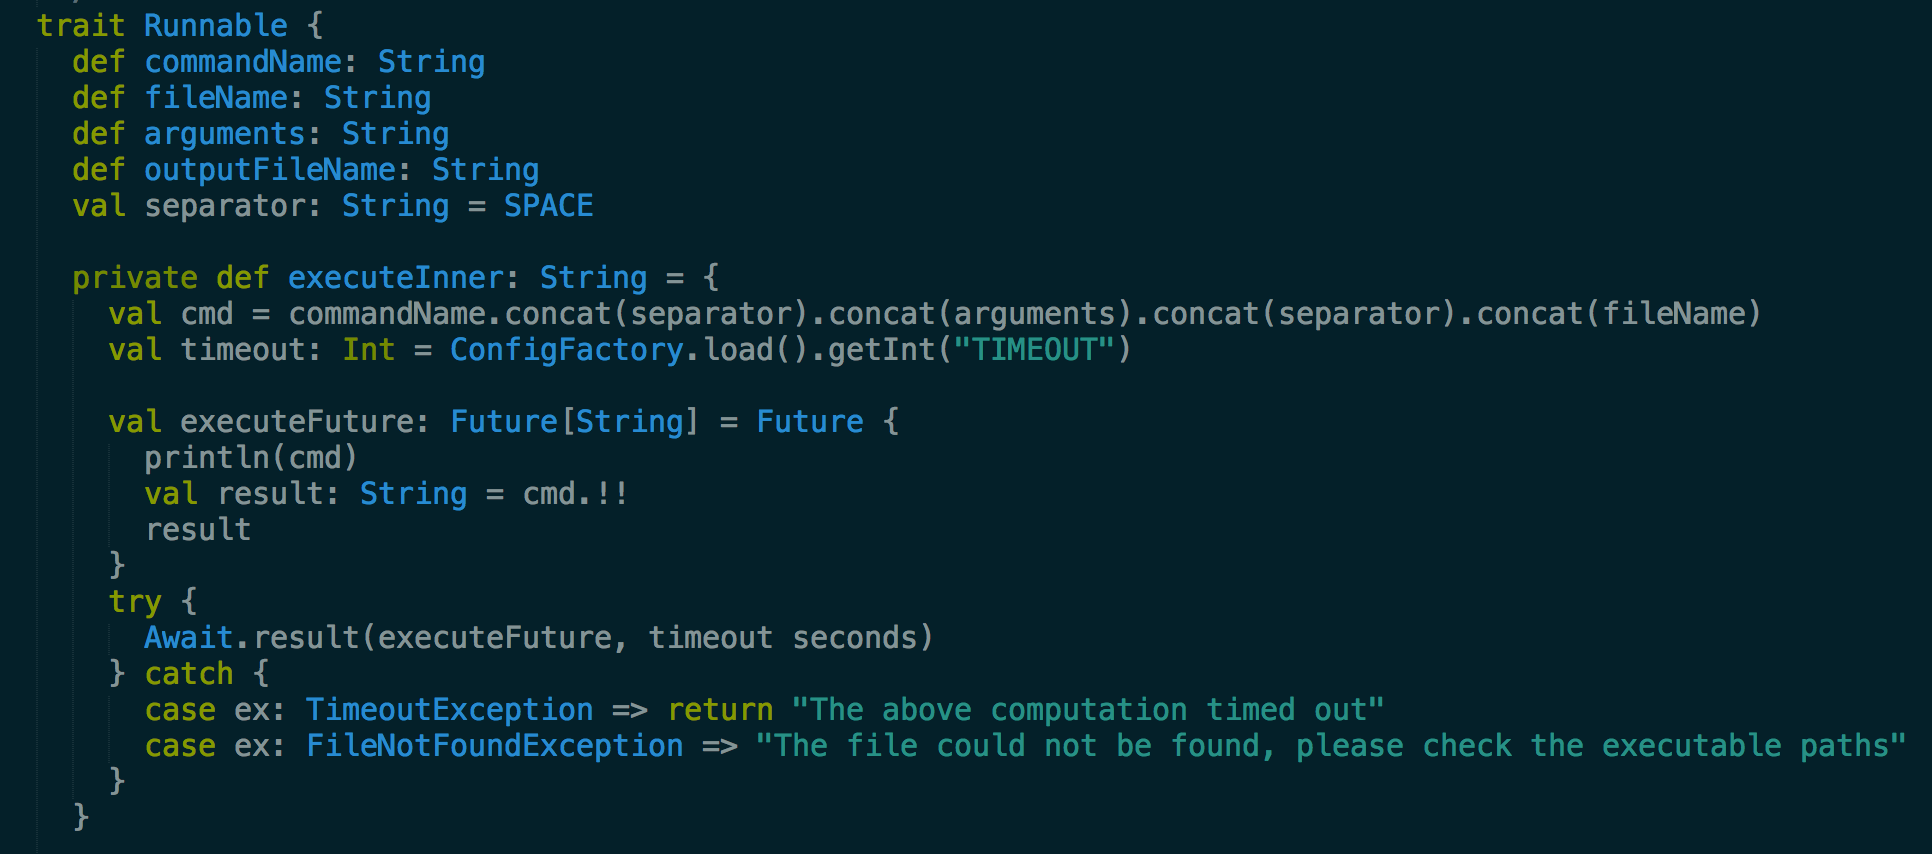
\includegraphics[width=500px]{figures/futures.png}
  \caption{An example of "Future Timeout" pattern usage}
\end{figure}
\item \textbf{Dependency Injection (DI) Pattern} - In software engineering, dependency injection is a software design pattern that implements inversion of control for software components. DI has been applied throughout the project to reduce coupling and make the code as extensible as possible. For example, \textbf{constructor injection} is performed for configuration type objects where custom configurations are possible.
\end{itemize}

\noindent
Fowler's concept of the "Fluent Interface" can be extended to Scala which models behaviour using traits rather than interfaces \cite{scala}. This in conjunction with the builder pattern lead to a declarative syntax. One of the uses of the builder is shown below.

\begin{figure}[H]
  \centering
    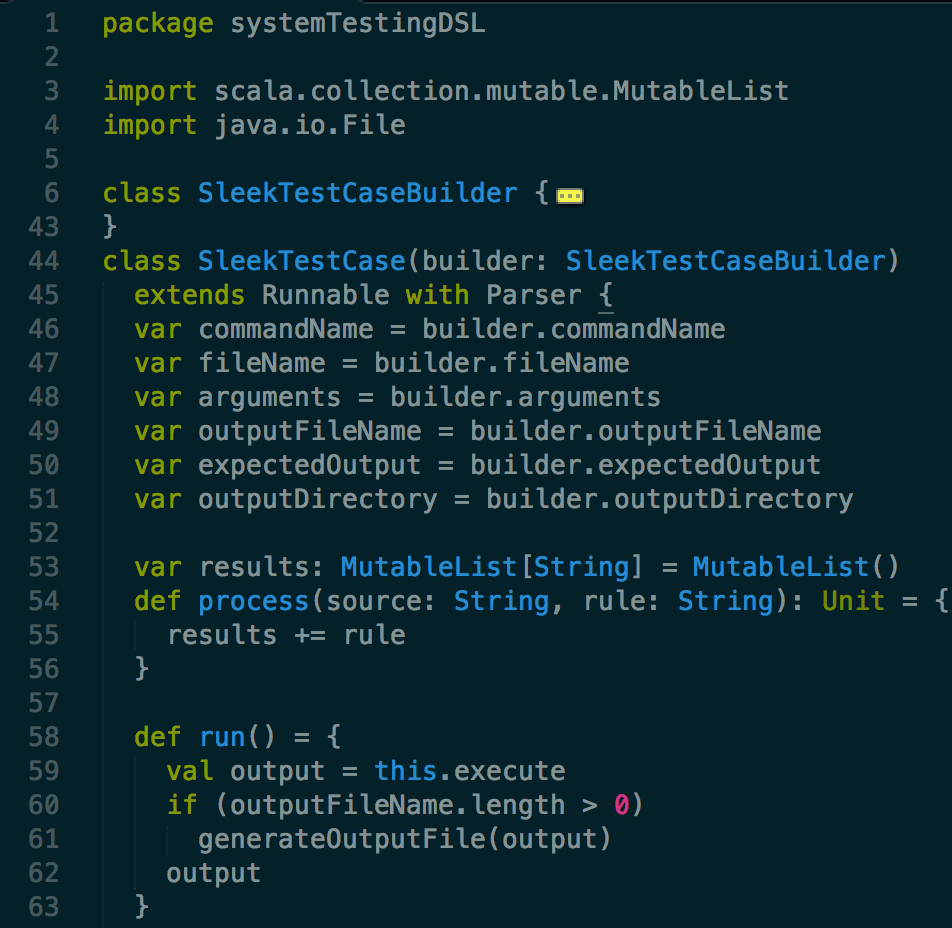
\includegraphics[width=300px]{figures/builder_pattern.png}
  \caption{An example of builder pattern usage}
\end{figure}

\subsection{Configuration Media}

The testing system that comprises the \textbf{Scala DSL} and the \textbf{Python Reporting Tool} require configuration in a human - readable format so that developers can conveniently integrated them into the testing work - flow. To keep both systems decoupled, they each have a configuration file. The Scala DSL can be configured by modifying \textbf{src/main/resources/application.conf} whereas the Python reporting tool can be configured by modifying \textbf{Reporting Tool/settings.yaml}.
\bigskip

\noindent
\textbf{Configuring the Scala DSL} - The \textit{application.conf} file contains settings specific to the HIP/SLEEK verification systems, regression test construction and regression test execution. Some general system level settings such as output file extensions and time - outs are also specified.
\bigskip

\noindent
\textbf{Configuring the Python Reporting Tool} - The \textit{settings.yaml} file in the Reporting Tool directory must be modified to configure the tool. The reason \textbf{YAML - Yet Another Markup Language} was chosen was to ensure \textbf{human - readability} and \textbf{conciseness}. A language like XML would have been verbose and more difficult to read for developers.

\begin{figure}[H]
  \centering
    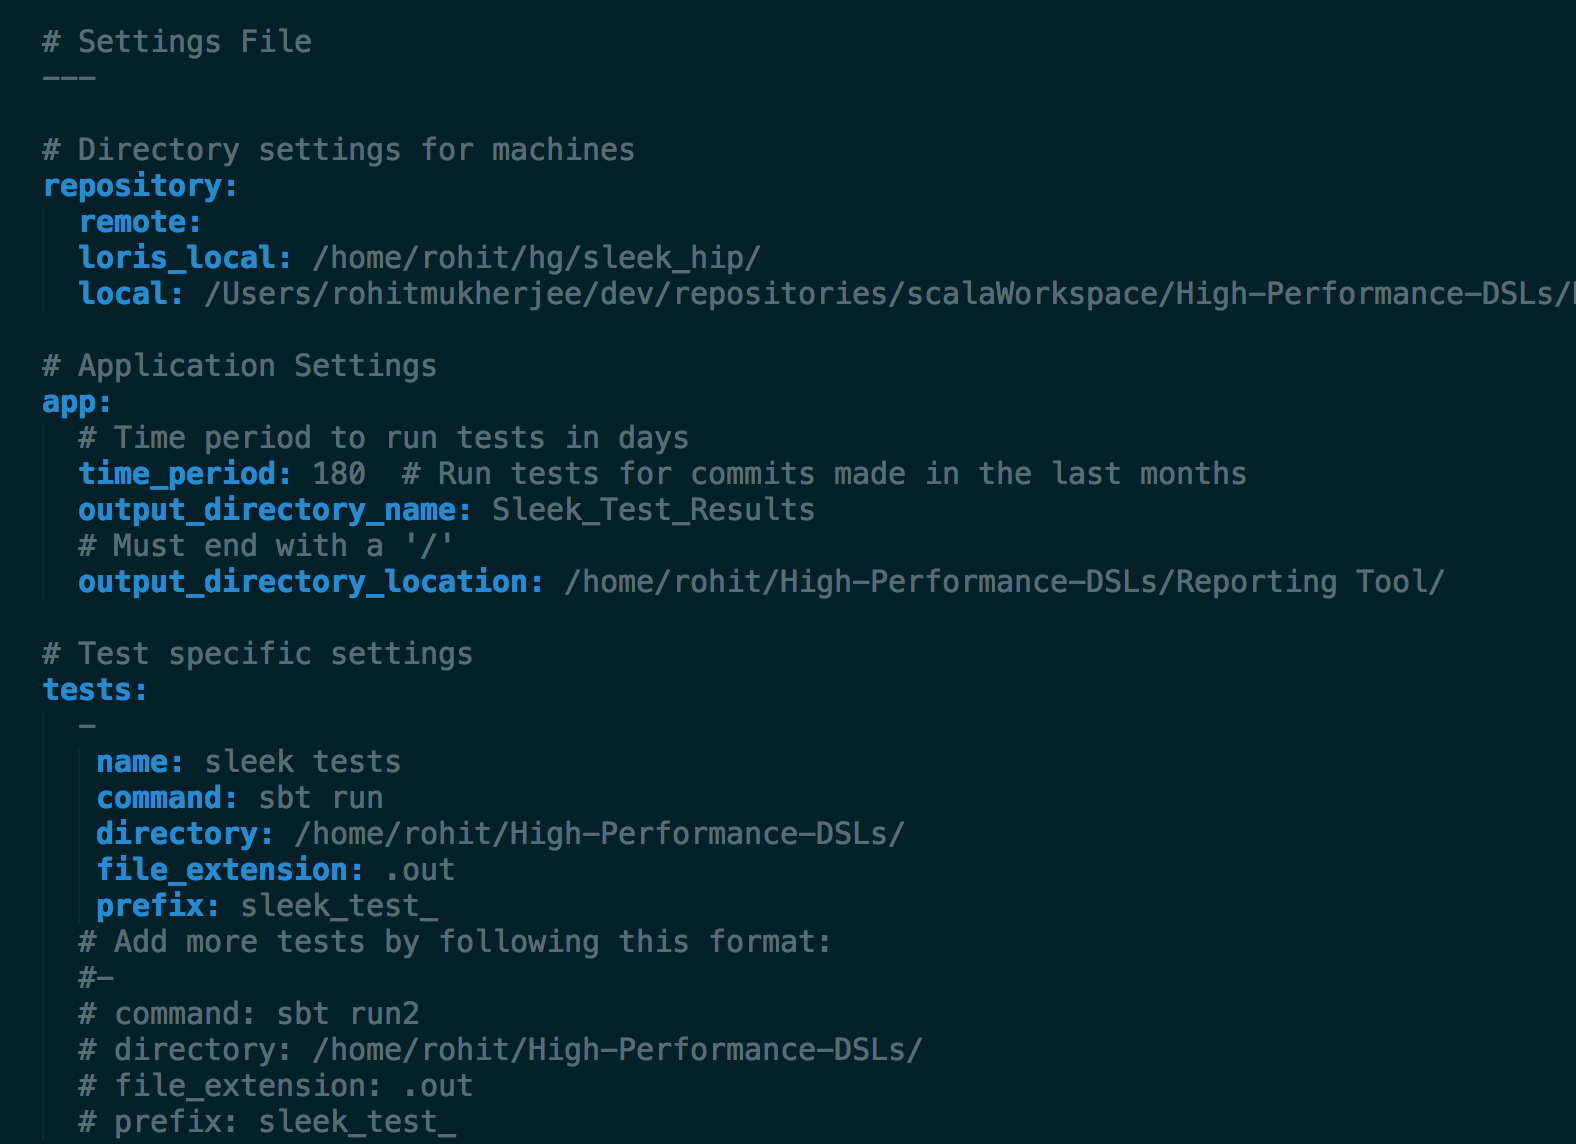
\includegraphics[width=500px]{figures/settings.png}
  \caption{settings.yaml - used to configure the reporting tool}
\end{figure}

\subsection{Deployment/Build Choices}
The entire project is managed using \textbf{Simple Build Tool} or sbt. SBT is itself a DSL and interactive build tool which supports parallel running of tests/build tasks. The following options are supported by the system \cite{sbt}. SBT was used because it is commonly used in industry to build and manage dependencies in Scala projects. It exports the compiled sources in .jar format allowing easy use in the form of a library.
\begin{itemize}
\item \textbf{sbt "run sleek"} - Executes all sleek tests
\item \textbf{sbt "run hip"} - Executes all hip tests
\item \textbf{sbt "run buildReference"} - Constructs references for regression testing
\item \textbf{sbt "run runReference"} - Runs tests against constructed references
\item \textbf{sbt "run overrideReference"} - Re - processes references
\item \textbf{sbt "run test"} - Executes unit tests written during development process.
\item \textbf{sbt "run help"} - Shows supported operations
\end{itemize}
\newpage

\section{Overview of Code}

An overview of the convenience methods/types exposed in the Scala DSL and the API of the Python system are shown below. Private and Protected members have not been shown and test packages/code have been excluded from the section in the interest of brevity. Building both projects with tests should show the test status.

\subsection{Scala Code Base}
A diagram of the Scala code base is shown below. Scala does not have tooling support for UML generation but allows diagrams like the one below to be generated. The shapes in \textbf{green} represent \textbf{types}, \textbf{orange} represents composite pattern usage or \textbf{client relationships} and \textbf{pink} represents \textbf{inheritance}.

\begin{figure}[H]
  \centering
    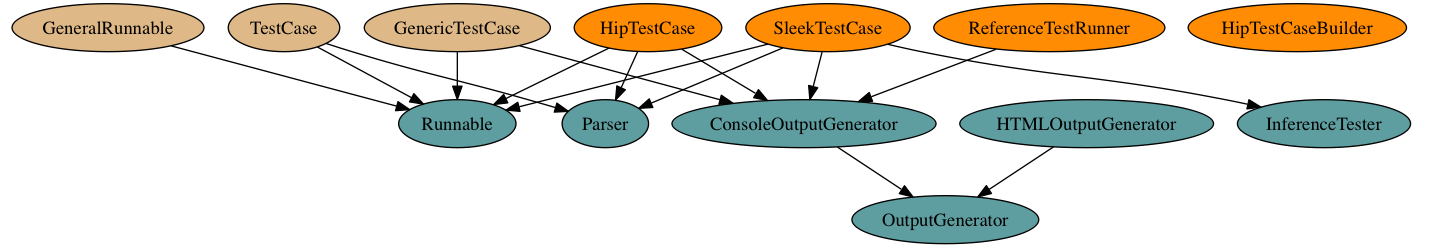
\includegraphics[height=80px]{figures/scala_uml.png}
  \caption{Overview of code base}
\end{figure}
\begin{itemize}

\item package systemTestingDSL
    \begin{itemize}
        \item \textbf{Object FileSystemUtilities} - Object with utility file system manipulation methods
        \item \textbf{Trait Runnable} - Models behaviour of any executable/command that can be run
        \item \textbf{Case Class General Runnable} - Models implementation of any executable/command 
        \item \textbf{Case Generic Test Case} - Test Case for any generic purpose runnable
        \item \textbf{Case Class HipTestCase} - Test Case especially for Hip verification
        \item \textbf{Object HipTestCaseUsage} - Client with hip test cases
        \item \textbf{Object HipTestSuiteUsage} - Client with hip test suites
        \item \textbf{Object SleekTestSuiteUsage} - Client with sleek test suites
        \item \textbf{Object SleekTestCaseUsage} - Client with sleek test cases
        \item \textbf{Object InferenceDefaults} - Sensible defaults for inference checking
        \item \textbf{Trait InferenceTester} - Trait with functionality to verify (a,b) tuples
        \item \textbf{Object Main} - This is passed arguments by sbt and contains factory methods
        \item \textbf{Trait Parser} - Regex and rule based parser methods are described here
        \item \textbf{Class ReferenceTestRunner} - Runs regression tests
        \item \textbf{Class RegressionTestReferenceBuilder} - Constructs regression tests
        \item \textbf{Case Class SleekTestCase} - Test Case especially for Sleek verification
        \item \textbf{Case Class TestCase} - Any Test Case
        \item \textbf{Case Class GenericTestSuite} - Automated testing of files of a certain type found          using regex matching
        
    \end{itemize}
\item package systemTestingDSL.outputGenerator
    \begin{itemize}
        \item \textbf{Trait OutputGenerator} - Specifies contract for output generation including logging, error, expected and success
        \item \textbf{Trait ConsoleOutputGenerator} - Mixin with methods which implement OutputGenerator's methods for console output
        \item \textbf{Trait HTMLOutputGenerator} - Mixin with methods which implement OutputGenerator's methods for HTML output
    \end{itemize}
\item package systemTestingDSL.matchers
    \begin{itemize}
    \item \textbf{Trait Matcher} - Models behaviour for any generic matcher
    \item \textbf{DiffMatcher} - Matches two files based on their diff
    \end{itemize}
\item package systemTestingDSL.testSuite
    \begin{itemize}
    \item \textbf{Case Class HipTestSuite} - Suite of hip test cases
    \item \textbf{Case Class SleekTestSuite} - Suite of sleek test cases
    \end{itemize}
\end{itemize}

\subsection{Python Code Base}
Diagrams of the Python code base is shown below. The first diagram captures the UML of the system and only shows portion of the code (parts that are object oriented). The second shows the \textbf{package diagram} with dependency information. The reason they are different is because a part of the tool is written in scripting style and the remaining in object oriented style. This also adequately reflects the versatility of a dynamic language such as Python.

\begin{figure}[H]
  \centering
    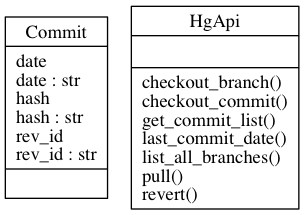
\includegraphics[height=150px]{figures/classes_reporting_tool.png}
  \caption{UML diagram for Reporting Tool}
\end{figure}

\noindent
An API for the Distributed Version Control System (DVCS) Mercurial, had to be written because the Mercurial team stated that their current API is being overhauled. The API developed implements a subset of the full command set based on usage. It is written as a wrapper around terminal commands.

\begin{figure}[H]
  \centering
    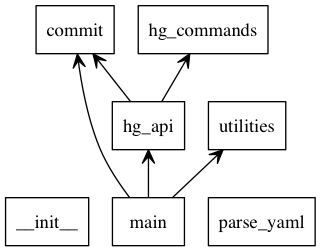
\includegraphics[height=150px]{figures/packages_reporting_tool.png}
  \caption{Package diagrams showing dependency graph for Reporting Tool}
\end{figure}

% \newpage
% \section{Current Applications of DSL/Reporting System}
% The goal for this semester was to read and apply the methods mentioned in literature and build a DSL that can be used for system testing. This process helped understand some of the patterns that can be applied in internal DSLs, requirements and specifications of the DSL itself and usage scenarios.
% \subsection{Regression Testing}
% \subsection{Sleek/Hip Verification}
% \subsection{Reporting/Scheduling features}
% \subsection{Integration with cron and tmux}
% \subsection{Other possible applications}
% \subsection{Deployment onto new systems} 
\newpage
\section{Conclusion}
\subsection{Summary of work}
Over the course of the project, the following tools were built:
\begin{itemize}
\item An extensible DSL for functional testing on a system level
\item Various source code translators to convert code from the Perl Script (run-fast-tests.pl) to the DSL code
\item A reporting tool in Python to test various branches/commits and produce hierarchical output
\item An API for Mercurial
\item Various techniques for DSL construction of DSLs.
\end{itemize}
\subsection{Goals achieved}
The following goals were achieved over the course of the final year project:
\begin{itemize}
\item Different approaches towards developing a scalable DSL were explored
\item An embedded DSL for system testing was developed using Scala
\item 3 applications of the system were found - \textbf{HIP Verification, SLEEK verification and Regression Testing}
\item A Reporting Tool was developed in Python which can test all branches/commits of a mercurial project and summarize the results in an organized manner
\item This reporting tool is highly configurable using a YAML settings file.
\item The old system performing HIP/SLEEK testing was a 2500 line Perl Script. All the source code was translated using \textit{source code translators in Python} to the DSL code.
\end{itemize}

\subsection{Future Work/Extension}
There are several areas of extension and improvement for the DSL developed over the last year. Some of these possible improvements are:
\begin{itemize}
\item Support for Unit Testing
\item Improvement of Performance Testing features
\item Cleaner syntax that abstracts away more details of host language, Scala
\item Run - time performance optimization through some meta - programming
\item Integrate \textbf{Git, SVN} or other version control tools with the reporting tool in Python
\item Set up an email server to email out bug reports when tests fail. This would give the reporting tool some features of a \textit{continuous integration} system.
\end{itemize}

\subsection{Project Statistics}

Some interesting statistics during the development process are:
\begin{itemize}
\item 80\% of the project is written in Scala
\item 10\% of the project is written in Python
\item The remaining 10\% comprises setup scripts, configuration files and documentation
\item The total number of lines of code in the system are approximately 10,000
\item The project has 7 branches and 199 commits in the master branch
\end{itemize}

A graph showing commit frequency between September and April is shown below:
\begin{figure}[H]
  \centering
    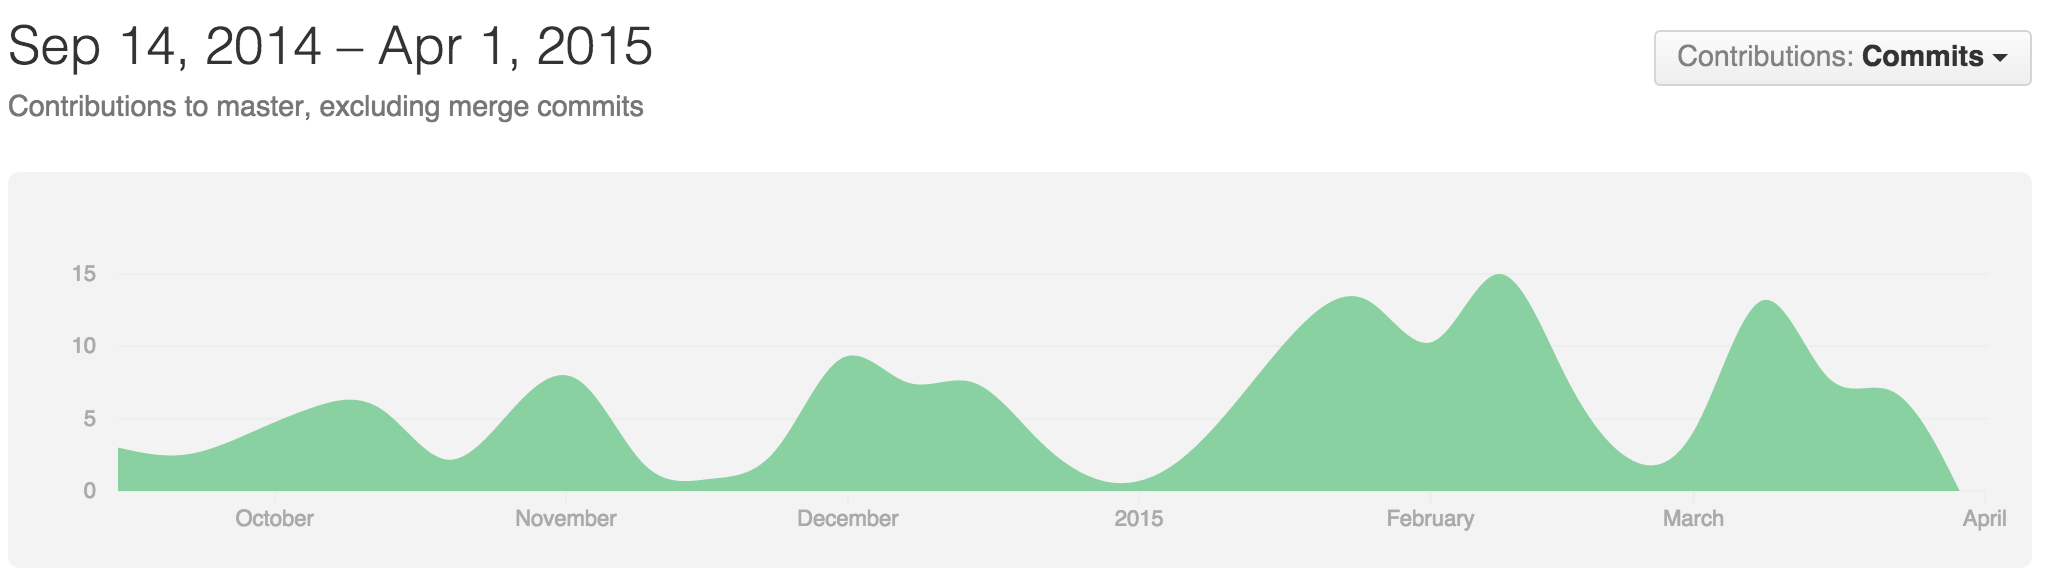
\includegraphics[height=150px]{figures/commit_frequency.png}
  \caption{Commit Frequency Statistics generated by Github}
\end{figure}
\newpage

\begin{thebibliography}{9}

\bibitem{hipsleek} Chin, W. (2011, January 1). http:\/\/cristian.pl-bits.ro/Publications/OOPSLA-Comp\_2011\_demo.pdf. Retrieved March 31, 2015, from http:\/\/cristian.pl-bits.ro/Publications/OOPSLA-Comp\_2011\_demo.pdf

\bibitem{agile} Dingsøyr, T., Nerur, S., Balijepally, V. and Moe, N. (2012). A decade of agile methodologies: Towards explaining agile software development. Journal of Systems and Software, 85(6), pp.1213-1221.
\bibitem{fluentInterface} Fowler, M. (2005, 12 20). Fluent interface. 
Retrieved from http://martinfowler.com/bliki/FluentInterface.html

\bibitem{dslsInAction}Ghosh, D. (2011). DSLs in Action (1st ed., pp. 20 - 87). Connecticut: Manning.

\bibitem{Hetzel88} Hetzel, William C., The Complete Guide to Software Testing, 2nd ed. Publication info: Wellesley, Mass. : QED Information Sciences, 1988. ISBN: 0894352423.Physical description: ix, 280 p. : ill ; 24 cm.

\bibitem{performanceComparison}Hundt, R. (2011, June 6). Loop Recognition in C /Java/Go/Scala. Retrieved March 30, 2015.
\bibitem{tdd} Introduction to Test Driven Development (TDD). (n.d.). Retrieved November 4, 2014.

\bibitem{lund} Lejdfors/Lund University, C. (2006). Techniques for implementing embedded domain specific languages in dynamic languages (Doctoral dissertation, Lund University, Lund, Sweden).

\bibitem{lms} Odersky, M., \& Rompf, T. (n.d.). Lightweight Modular Staging: 
A Pragmatic Approach to Runtime ode Generation and Compiled DSLs. \textit{GPCE 2010, October 10–13, 2010}. Retrieved from http://infoscience.epfl.ch/record/150347/files/gpce63-rompf.pdf

\bibitem{delite} Odersky, M., \& Sujeeth, A. (2013). Forge: Generating a 
High Performance DSL Implementation from a Declarative Specification. \textit{GPCE 2013: 12th International Conference on Generative Programming: Concepts \& Experiences}. 
Retrieved November 4, 2014, from http://ppl.stanford.edu/papers/gpce13-sujeeth.pdf

\bibitem{sbt} The interactive build tool (sbt) http://www.scala-sbt.org/
\bibitem{python}The Python Programming Language. (n.d.). Retrieved March 31, 2015, from https://www.python.org/doc/
\bibitem{scala} The Scala Programming Language (The Scala Programming Language)

\bibitem{unitTestingAtMicrosoft} Williams, L., Kudrjavets, G., \& Nagappan, N. (2008). On the Effectiveness of Unit Test Automation at Microsoft.
http://www.scala-lang.org/
\end{thebibliography}
\end{document}